\chapter{Recherche de résonances de spin 1 dans le spectre de masse \ttbar} \label{chap:zprime}

Ce chapitre est consacré entièrement à la recherche de résonance de spin 1 dans le spectre de masse \ttbar. Plusieurs modèles (topcolor, dimensions supplémentaires, etc.) prédisent de nouvelles particules de spin 1 se manifestant comme des résonances dans le spectre \mtt (voir \cref{chap:new_physics} pour plus de détails).

\bigskip

Plus spécifiquement, cette analyse se concentre sur la recherche de \zprime, boson neutre massif, ainsi que sur la recherche d'excitations de Kaluza-Klein du gluon, dans le modèle Randall-Sundrum. Néanmoins, on verra par la suite qu'un effort particulier a été fait pour rendre l'analyse indépendante du modèle théorique considéré.

\section{Signaux et bruits de fonds}

Afin d'être en mesure de confronter aux mesures expérimentales le plus grand nombre possible de modèles théorique, on souhaite rester le plus possible indépendant d'un modèle quelconque. Pour cela, on modélise le signal par une résonance générique, dont la largeur est fixée arbitrairement, tout comme la section efficace. Afin de couvrir une vaste gamme de modèles théoriques, deux types de résonances sont modélisées :
\begin{itemize}
    \item Les résonances étroites, avec une largeur $\sigma = \num{0.01} \, \mzp$, plus faible que la résolution expérimentale sur la reconstruction de la masse invariante \ttbar.
    \item Les résonances larges, avec une largeur $\sigma = \num{0.10} \, \mzp$, équivalent à la résolution expérimentale sur la reconstruction de la masse invariante \ttbar.
\end{itemize}

Ces résonances sont générées à l'aide de \texttt{MadGraph 4}, en utilisant un modèle de \zprime générique. Dans ce modèle, le \zprime possède les même couplages fermioniques que le boson \PZ du Modèle Standard, et la rapport d'embranchement en \ttbar est fixé à \SI{100}{\%}. Plusieurs masses sont générées, allant de \SI{500}{\GeV} à \SI{2}{\TeV}, par pas de \SI{250}{\GeV} (excepté \SI{1750}{\GeV}).

\smallskip

En plus de résonances \zprime génériques, on génère en plus des résonances selon un modèle théorique particulier d'excitations de Kaluza-Klein du gluon à l'aide de \texttt{Pythia 8}. Dans ce modèle, la largeur de la résonance ainsi que la section efficace sont fixées par la masse de la résonance.

\medskip

La \cref{fig:mtt_gen} présente les distributions de masse invariante \ttbar pour chacune des résonances simulées.

\begin{figure}[tbp] \centering
    \subcaptionbox{\zprime étroit}[0.33\textwidth]{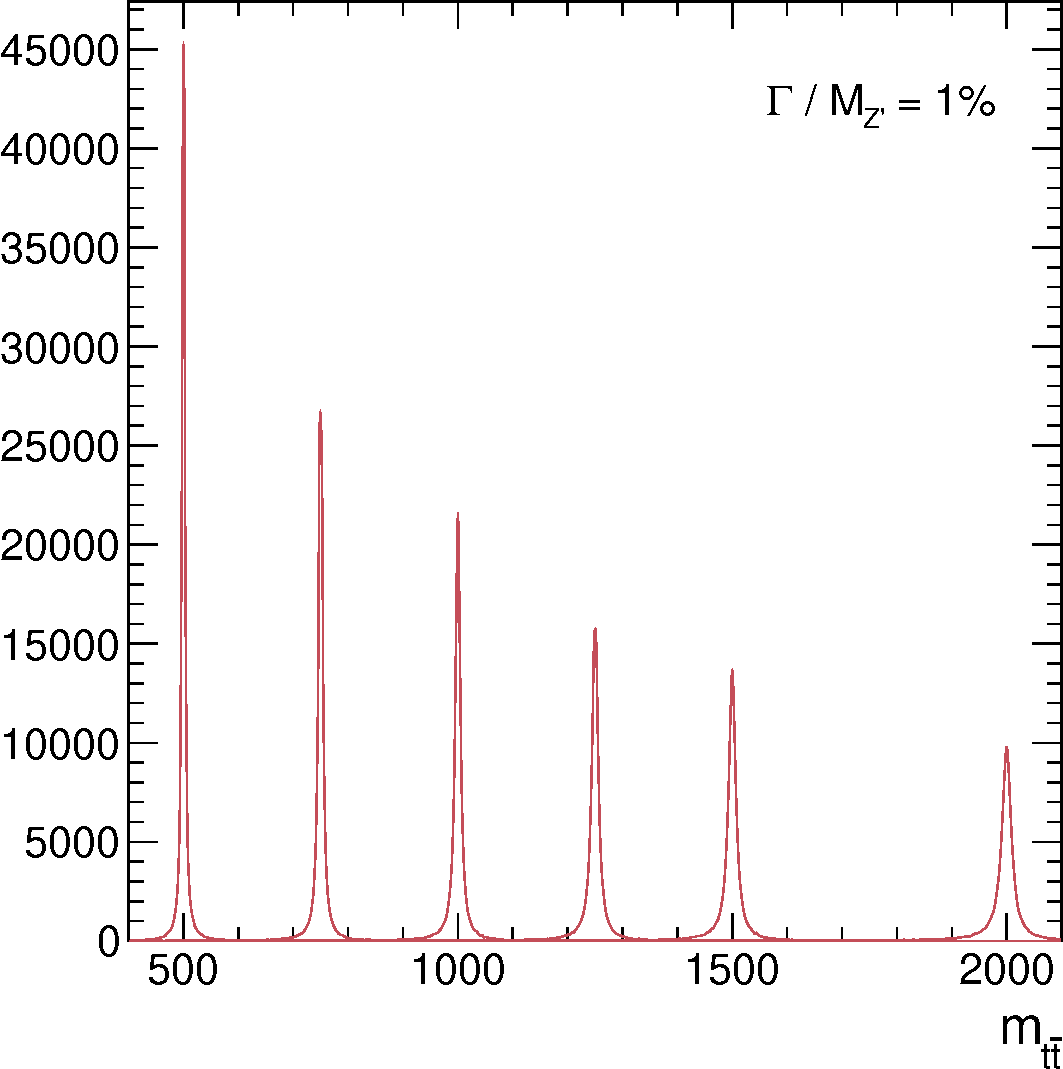
\includegraphics[width=0.33\textwidth]{chapitre7/figs/mtt_zprime_narrow_gen.pdf}}
    \subcaptionbox{\zprime large}[0.33\textwidth]{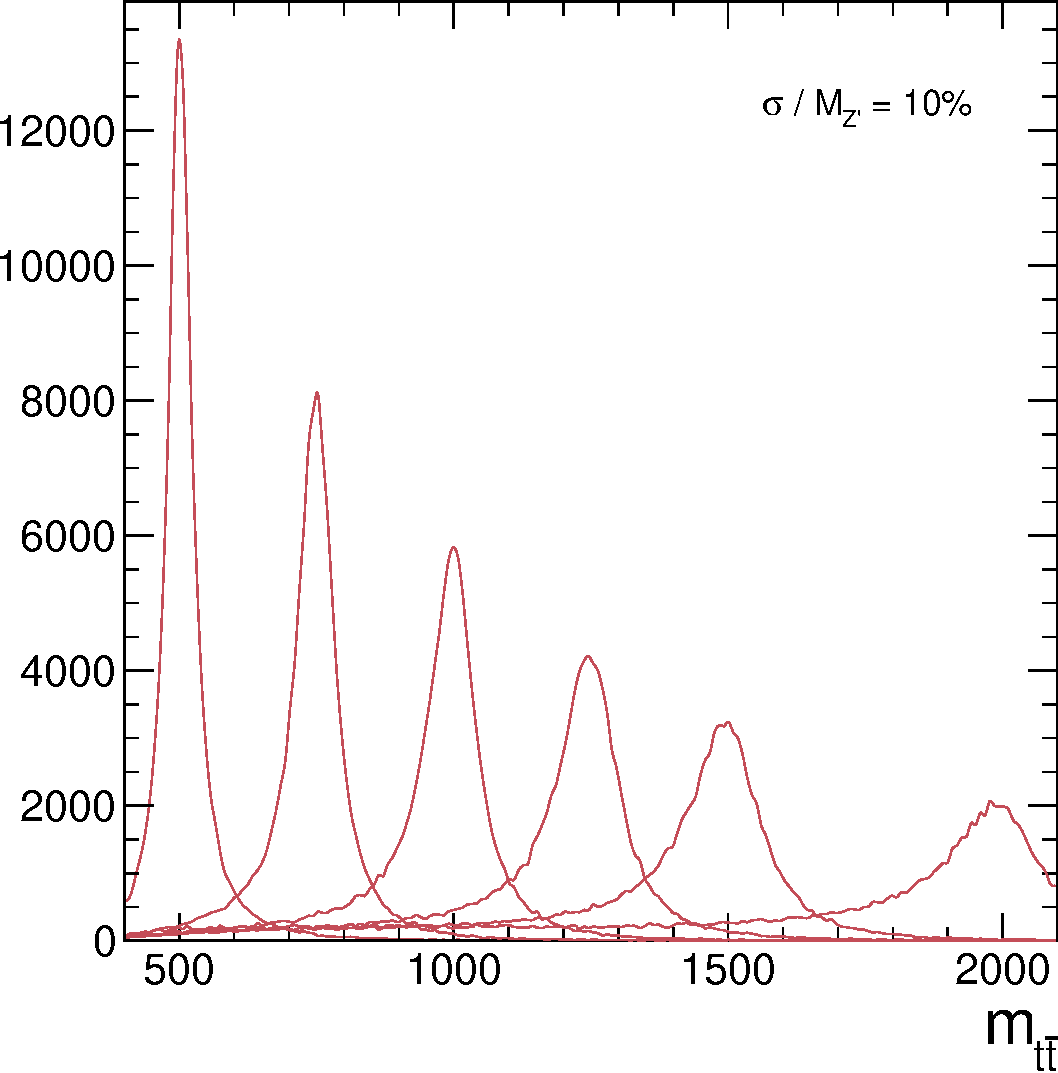
\includegraphics[width=0.33\textwidth]{chapitre7/figs/mtt_zprime_large_gen.pdf}}
    \subcaptionbox{\kkglu}[0.325\textwidth]{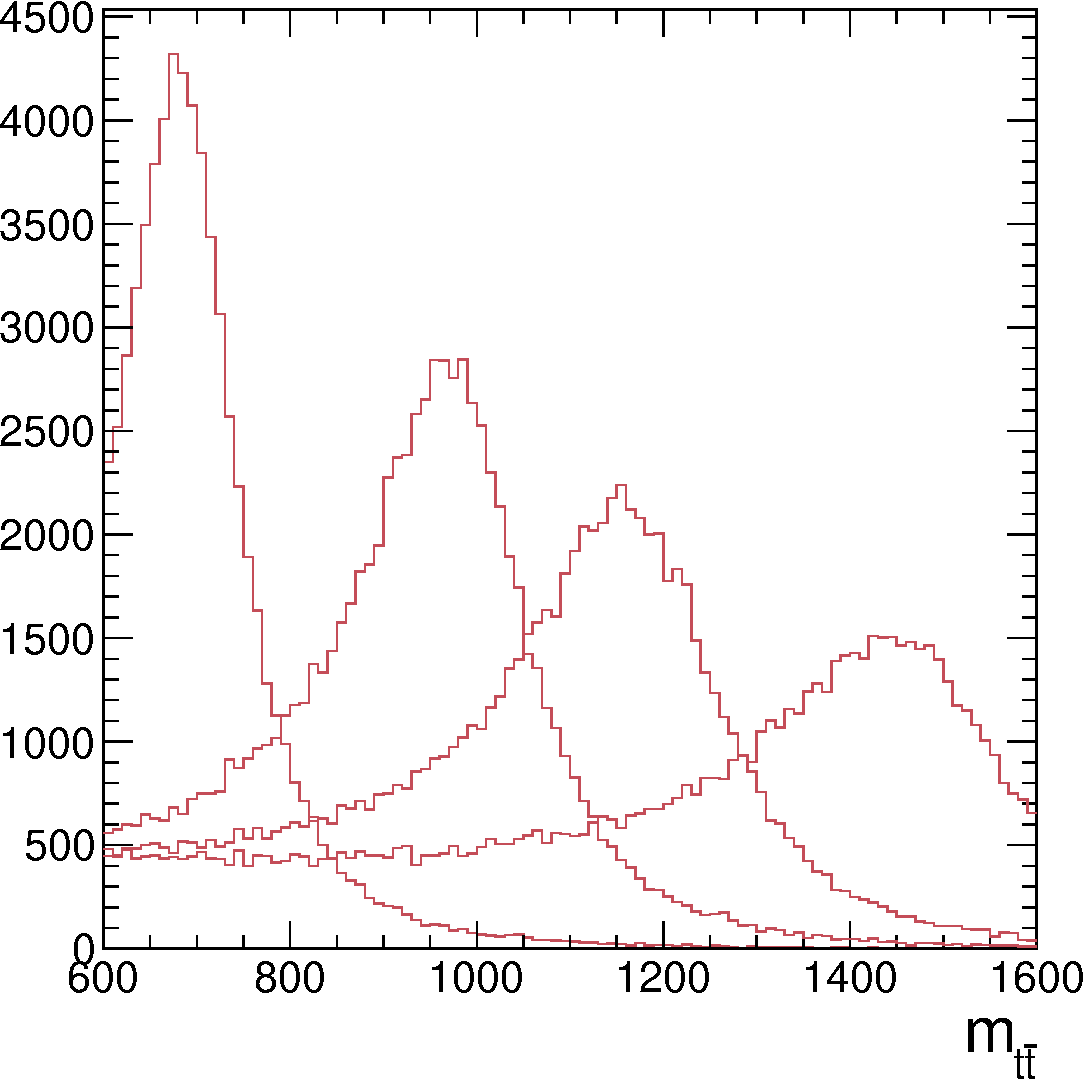
\includegraphics[width=0.325\textwidth]{chapitre7/figs/mtt_rsgluons_gen.pdf}}
    \caption{Masse invariante \ttbar pour chaque point de signal généré.}
    \label{fig:mtt_gen}
\end{figure}

\bigskip

L'analyse se concentre exclusivement le canal de désintégration des paires \ttbar semi-leptonique, pour plusieurs raisons :
\begin{itemize}
    \item Le rapport d'embranchement dans ce canal est \tilde\SI{44}{\%}, contre \SI{11}{\%} pour le canal di-leptonique, et \SI{45}{\%} pour le canal tout-hadronique.
    \item La présence d'un lepton constitue une signature expérimentale claire. L'avantage par rapport au canal di-leptonique, outre le rapport d'embranchement, vient de l'absence d'ambiguïté pour le choix du neutrino, améliorant la résolution de reconstruction.
    \item L'absence de neutrino dans le canal tout-hadronique est compensé par la nécessitée de correctement sélectionner les 6 bons jets provenant de la désintégration \ttbar.
\end{itemize}

Expérimentalement, une telle désintégration se traduit par la présence d'un lepton isolé, de 4 jets, et de l'énergie transverse manquante (neutrino). Tous les processus physique du Modèle Standard produisant des états finaux similaires sont considérés comme des bruits de fond. Le fond le plus important est bien évidemment la production de paires \ttbar du Modèle Standard, bruit de fond irréductible. Les autres bruits de fond considérés sont :
\begin{itemize}
    \item La production d'un boson \PW avec des jets associés (\PW + jets).
    \item La production d'un boson \PZ avec des jets associés (\PZ + jets) : un des leptons provenant de la désintégration du \PZ est mal identifié.
    \item La production d'un quark top célibataire.
\end{itemize}

D'autres processus entrent aussi dans la composition du bruit de fond, tels que les événements multi-jets ou di-bosons (\PW{}\PW, \PZ{}\PZ, \PW{}\PZ). Après notre sélection, le nombre d'événement provenant de ces fonds est très largement minoritaire face aux autres fonds. Ils ne sont donc pas inclus dans notre analyse. Le \cref{tab:backgrounds} liste les sections efficaces de chaque bruit de fond considéré, ainsi que la luminosité équivalente disponible pour l'analyse.

\begin{table} \centering
  \begin{tabular}{@{}ccc@{}} \toprule
    Processus & Section efficace (\si{\pb}) & Luminosité équivalente (\si{\invfb}) \\ \midrule
    \ttbar & \num{245.8} (NNLO) & \num{84.34} \\
    \PW + jets & \num{37509} (NNLO) & \num{1.54} \\
    \PZ + jets & \num{3504} (NNLO) & \num{8.69} \\
    Top célibataire (voie s) & \num{5,56} (NNLO appr.) & \num{71.96} \\
    Top célibataire (voie t) & \num{87,1} (NNLO appr.) & \num{65.37} \\
    Top célibataire (voie t\PW) & \num{22.35} (NNLO appr.) & \num{44.34} \\ \bottomrule
  \end{tabular}
  \caption{Section efficace et luminosité équivalente pour chacun des bruits de fond considérés.}
  \label{tab:backgrounds}
\end{table}

\section{Sélection des événements}

On souhaite sélectionner des événements compatible avec la désintégration semi-leptonique de paires \ttbar, c'est-à-dire comprenant un lepton isolé, au moins 4 jets et de l'énergie transverse manquante. On applique pour cela une série de coupures afin de réduire le plus possible le bruit de fond tout en gardant un maximum d'événements de signal.

\medskip

Chaque événement est catégorisé selon la saveur du lepton. On définit ainsi le canal semi-muonique (semi-$\mu$), lorsque le lepton isolé est un muon, et le canal semi-électronique (semi-e) lorsque c'est un électron.

\subsection{Identification des objets}

L'événement est reconstruit à l'aide de l'algorithme du \pf, tel que décrit en détail dans le \cref{chap:reco}. Plusieurs étapes supplémentaires sont ajoutées à la reconstruction permettant de limiter les effets du \pu sur la reconstruction des jets :
\begin{itemize}
    \item On identifie les leptons isolés parmi les candidats \pf. Les critères d'isolation sont définis plus loin.
    \item On identifie ensuite les hadrons chargés provenant d'un vertex d'interaction autre que le vertex principal comme du \pu.
    \item L'agglomération des jets est ensuite effectuée avec les candidats \pf qui ne sont pas identifiés comme \pu ou leptons isolés.
\end{itemize}

% Comme mentionné précédemment, cette procédure permet de limité les effets du \pu sur la reconstruction des jets. En enlevant les leptons isolés de la reconstruction des jets, on évite tout problème de double comptage de l'énergie : le lepton utilisé n'est forcément dans aucun jet
L'isolation du lepton est définie par la relation
\begin{align*}
  I_{\Plepton} &= \frac{\sum{\pt^\text{hadrons chargés}} + \sum{\pt^\text{hadrons neutres}} + \sum{\pt^\text{photons}}}{\pt^{\Plepton}}
\end{align*}
où les sommes portent sur les particules contenues dans un cône de rayon $\Delta R$ centré autour du lepton. Ainsi, plus $I$ tend vers 0, plus la particule est isolée. Deux valeurs de $\Delta R$ sont utilisées, suivant la saveur du lepton :
\begin{align*}
  \Delta R &= \num{0.4} \quad\text{muons}\\
  \Delta R &= \num{0.3} \quad\text{électrons}
\end{align*}

Dans le cas des muons, la définition de l'isolation $I$ est modifiée afin d'être plus robuste face au \pu. La soustraction des hadrons chargés provenant de vertex secondaires n'est en effet pas suffisante, puisque les hadrons neutres ainsi que le \pu est aussi composé de hadrons neutres et de photons, et on estime qu'ils sont responsable d'environ la moitié de l'énergie provenant du \pu. Ainsi, on soustrait du calcul de l'isolation la moitié de l'énergie des hadrons provenant du \pu, en vérifiant bien que l'énergie provenant de la partie neutre ne soit jamais négative. On obtient alors
\begin{align*}
  I_{\Pmu}^\text{corrigé} &= \frac{\sum{\pt^\text{hadrons chargés}} + \overbrace{\left(\sum{\pt^\text{hadrons neutres}} + \sum{\pt^\text{photons}} - \num{0.5} \sum{\pt^\text{hadrons chargés \pu}} \right)}^{= 0 \text{ si négatif}}}{\pt^{\Plepton}}
\end{align*}
On considère un muon comme isolé si $I_{\Pmu}^\text{corrigé} < \SI{12}{\%}$.

Pour les électrons, on applique une procédure similaire. Néanmoins, au lieu de soustraire la moitié de l'énergie des hadrons chargés provenant du \pu, on estime l'énergie restant dû au \pu en utilisant la densité d'énergie dans l'événement par unité de surface ($\rho$, voir \cref{sec:jec_l1}). Au lieu d'utiliser la surface du cône d'isolation, parfois délicate à calculer géométriquement, pour estimer la quantité d'énergie du \pu, on évalue une surface effective ($EA$) sur des événements \PZ $\rightarrow$ \Pelectron{}\Ppositron. Cette surface est définie comme le rapport entre la pente de la droite $\rho = f(N_{\text{vertex}})$ et la pente de la droite $I = f(N_\text{vertex})$.
\begin{align*}
  I_{\Pe}^\text{corrigé} &= \frac{\sum{\pt^\text{hadrons chargés}} + \overbrace{\left(\sum{\pt^\text{hadrons neutres}} + \sum{\pt^\text{photons}} - \rho\,EA \right)}^{= 0 \text{ si négatif}}}{\pt^{\Plepton}}
\end{align*}
On considère un électron comme isolé si $I_{\Pe}^\text{corrigé} < \SI{10}{\%}$. Cette valeur est plus faible en raison de la taille du cône plus faible aussi.

\bigskip

Des critères de qualité sont appliqués aux muons et électrons \pf, afin de s'assurer de la qualité des objets utilisés dans l'analyse. Ces critères sont détaillés dans la suite de cette section. La sélection sera elle détaillée dans la prochaine section. Pour chaque saveur, deux jeux de critères sont définis : une sélection lâche, qui servira pour effectuer un veto sur la présence de leptons additionnels, et une sélection forte, utilisé pour sélectionner le lepton principal.

\subsubsection{Muons} \label{sec:sel_muon}

Afin d'être identifié comme \textbf{lâche}, un muon doit passer les coupures suivantes.
\begin{itemize}
    \item Le muon doit être reconstruit avec l'algorithme du \pf, et être soit \emph{tracker} ou global (voir \cref{sec:muon_reco}).
    \item L'isolation relative $I_{\Pmu}^\text{corrigé}$ doit être inférieure à \SI{20}{\%}.
    \item L'impulsion transverse doit être supérieur à \SI{10}{\GeV}, et $\aeta < \num{2.5}$.
\end{itemize}

En plus de ces coupures, on identifie un muon de qualité s'il vérifie les critères suivants :
\begin{itemize}
  \item Le muon doit être reconstruit avec l'algorithme du \pf, et être un muon global.
  \item L'isolation relative $I_{\Pmu}^\text{corrigé}$ doit être inférieure à \SI{12}{\%}.
  \item La valeur du $\chi^2$ de l'ajustement global de la trace du muon divisé par le nombre de degrés de liberté de l'ajustement doit être inférieure à \num{10}.
  \item Le nombre de \emph{hits} laissés par le muons dans les couches du trajectographe doit être au moins égal à 5, afin d'assurer une mesure précise de l'impulsion transverse.
  \item L'ajustement global de la trace doit inclure au moins un \emph{hit} dans les chambres à muons.
  % \item La distance longitudinale de la trace par rapport au vertex primaire doit être inférieure à \SI{0.5}{\cm}.
  % \item La distance du paramètre d'impact transverse par rapport au vertex primaire doit être inférieure à \SI{0.2}{\cm}.
  \item L'impulsion transverse du muon doit être supérieure à \SI{26}{\GeV}, et $\aeta < \num{2.1}$.
\end{itemize}

\begin{figure}[tbp] \centering
    \subcaptionbox{\label{fig:muon_id_eff}}[0.48\textwidth]{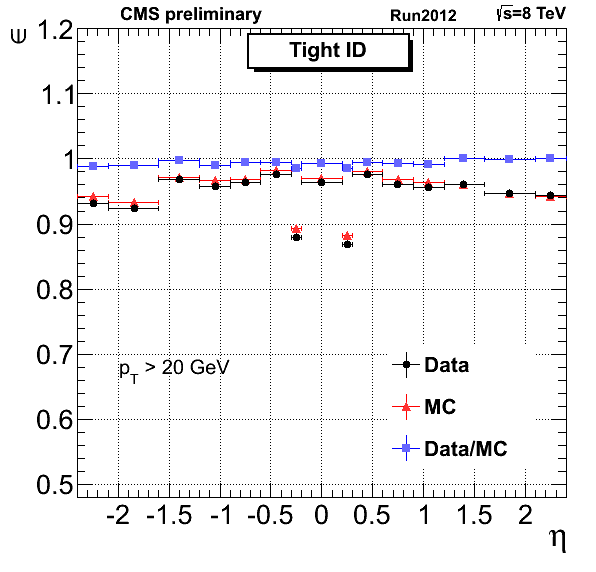
\includegraphics[width=0.48\textwidth]{chapitre7/figs/muon_id_efficiency.png}} \hfill
    \subcaptionbox{\label{fig:muon_iso_eff}}[0.48\textwidth]{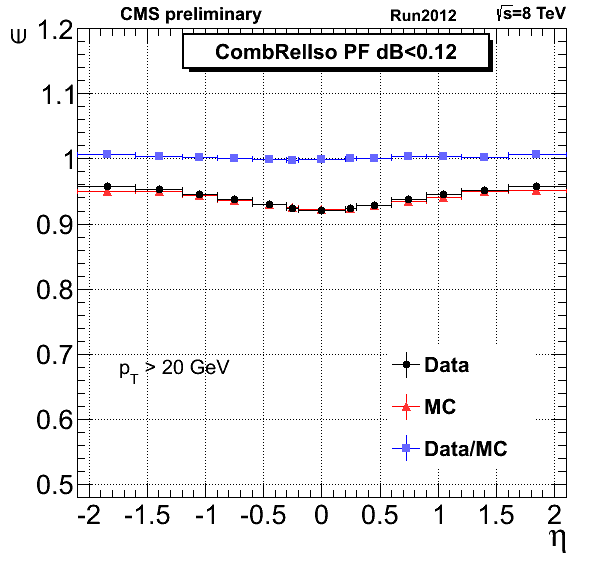
\includegraphics[width=0.48\textwidth]{chapitre7/figs/muon_iso_efficiency.png}}
    \caption{Efficacité de la sélection appliquée aux muons (\subref{fig:muon_id_eff}) ainsi que l'isolation (\subref{fig:muon_iso_eff}) en fonction de \aeta, pour les donnée (noir) ainsi que la simulation (rouge).}
\end{figure}

La \cref{fig:muon_id_eff} présente l'efficacité de cette sélection, qui varie entre \num{88} et \SI{98}{\%}. L'efficacité de l'isolation est-elle présentée sur la \cref{fig:muon_iso_eff}, et varie entre \num{92} et \SI{96}{\%}.

\subsubsection{Électrons} \label{sec:sel_electron}

\fxnote{Compléter cette section}

De façon analogue aux muons, on définit également deux jeux de critères pour identifier les électrons. Un électron est identifié comme \textbf{lâche} s'il passe les coupures suivantes :
\begin{itemize}
  \item L'électron doit être reconstruit avec l'algorithme du \pf.
\end{itemize}

On identifie un électron de qualité s'il vérifie les critères suivants :
\begin{itemize}
  \item L'électron doit être reconstruit avec l'algorithme du \pf.
\end{itemize}

\begin{figure}[htbp]
  \centering
  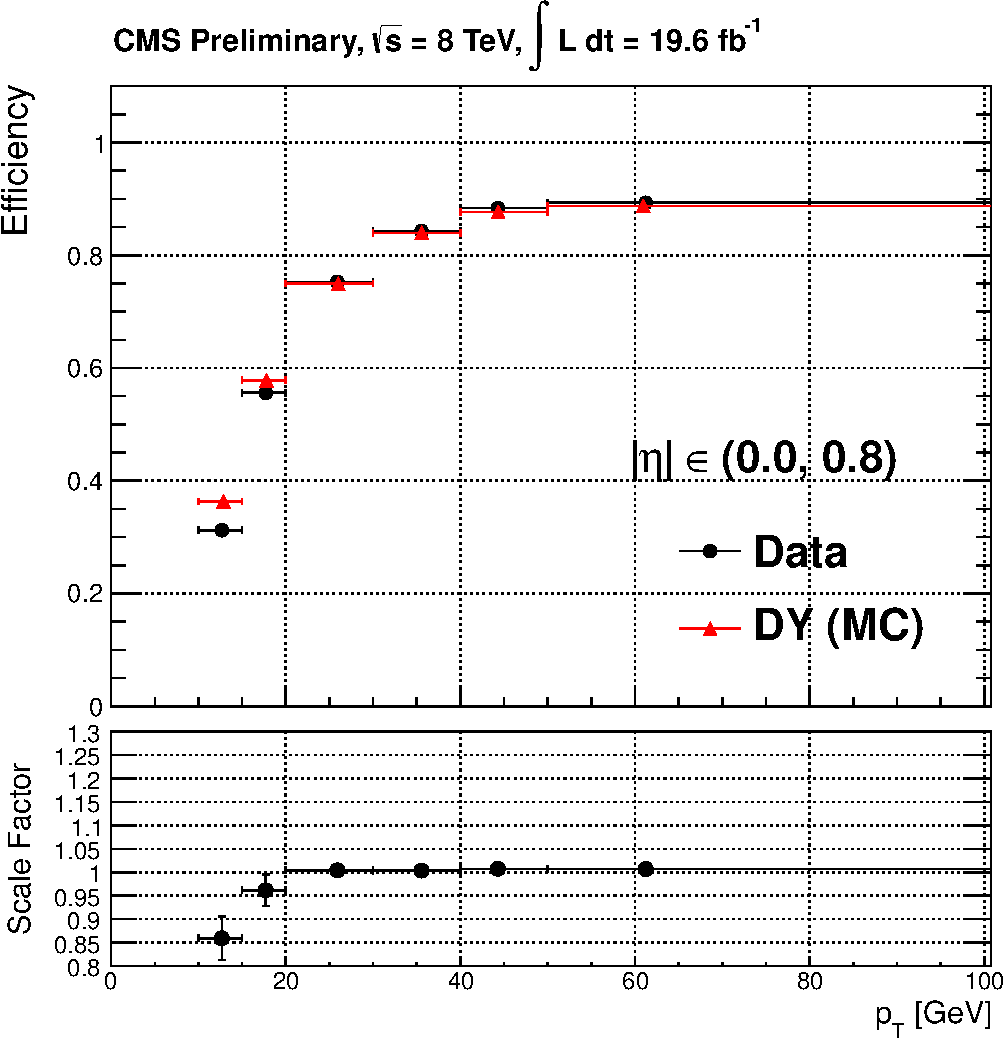
\includegraphics[width=0.6\textwidth]{chapitre7/figs/electron_id_eff.pdf}
  \caption{caption}
  \label{fig:label}
\end{figure}

\subsubsection{Jets}

Les jets sont reconstruits à l'aide de l'algorithme anti-$k_T$, avec une largeur de cône $R = \num{0.5}$ (voir \cref{sec:jet_reco}). Toutes les particules \pf n'étant ni des leptons isolés, ni du \pu sont utilisées dans l'agglomération des jets. Les corrections de niveaux 1, 2 et 3 sont appliquées, ainsi que les corrections résiduelles sur les données uniquement (plus de détails dans le \cref{chap:jetmet}).

On a évoqué rapidement dans le \cref{chap:jetmet} que la résolution des jets sur la simulation était meilleure que celle des jets reconstruits sur les données. On applique une série de corrections afin de dégrader la résolution des jets sur la simulation, afin de correspondre mieux à celle des données. L'impulsion transverse des jets est corrigé par un facteur $C$, définit par :
\begin{align*}
  C &= \max\left(0, 1 + \left[ 1 - \frac{\pt^\text{gen}}{\pt^\text{jet}} \right] \, f(\pt, \eta)\right)
\end{align*}
où $\pt^\text{jet}$ est l'impulsion transverse du jet, $\pt^\text{gen}$ est l'impulsion transverse du jet généré, et $f(\pt, \eta)$ un facteur de correction permettant de corriger la dégrader la résolution des jets. Les corrections en énergie et en résolution des jets sont propagées à l'énergie transverse manquante (voir \cref{sec:jetmet_sel}, \cpageref{page:met_propagation} pour plus détails sur la façon dont ces corrections sont propagées à l'énergie transverse manquante).

L'algorithme utilisé pour l'étiquetage des jets de \Pbottom est présenté en détails \cref{sec:b_tagging}. Afin d'éliminer les jets provenant des bruits des détecteurs, une sélection lâche est appliquée :
\begin{itemize}
  \item \fxerror{détailler}
\end{itemize}

Cette sélection a une efficacité supérieure à \SI{99}{\%}.

\subsubsection{Énergie transverse manquante}

L'énergie transverse manquante est reconstruite à l'aide de toutes les particules \pf de l'événement, comme décrit \cref{sec:met}. Toutes les corrections appliquées aux jets sont propagées à l'énergie transverse manquante.

\medskip

La distribution de l'énergie transverse manquante est isotrope en $\phi$ à cause d'une symétrie de rotation des collisions autour de l'axe $z$. Il est cependant observé sur les données qu'après reconstruction, la distribution de \phi de l'énergie transverse manquante n'est pas constante, mais présente une oscillation sinusoïdale de période \tilde$\num{2}\pi$. Cette oscillation peut avoir plusieurs causes, telle qu'une réponse anisotropique des détecteurs, des cellules calorimétriques inactives, un mauvais alignement des détecteurs, ainsi qu'un décalage du point d'interaction. On corrige cet effet, préjudiciable pour la reconstruction de la masse invariante, en décalant l'origine des coordonnées $x$ et $y$ :
\begin{align*}
  \METx &= \METx^\text{non corrigé} + c_x\\
  \METy &= \METy^\text{non corrigé} + c_y
\end{align*}
où $c_y$ et $c_y$ sont les facteurs de corrections, dérivées centralement par la collaboration. L'effet de cette correction est visible dans la \cref{fig:met_phi}.

\bigskip

\begin{figure}[tbp] \centering
    \subcaptionbox{\label{fig:met_phi}}[0.48\textwidth]{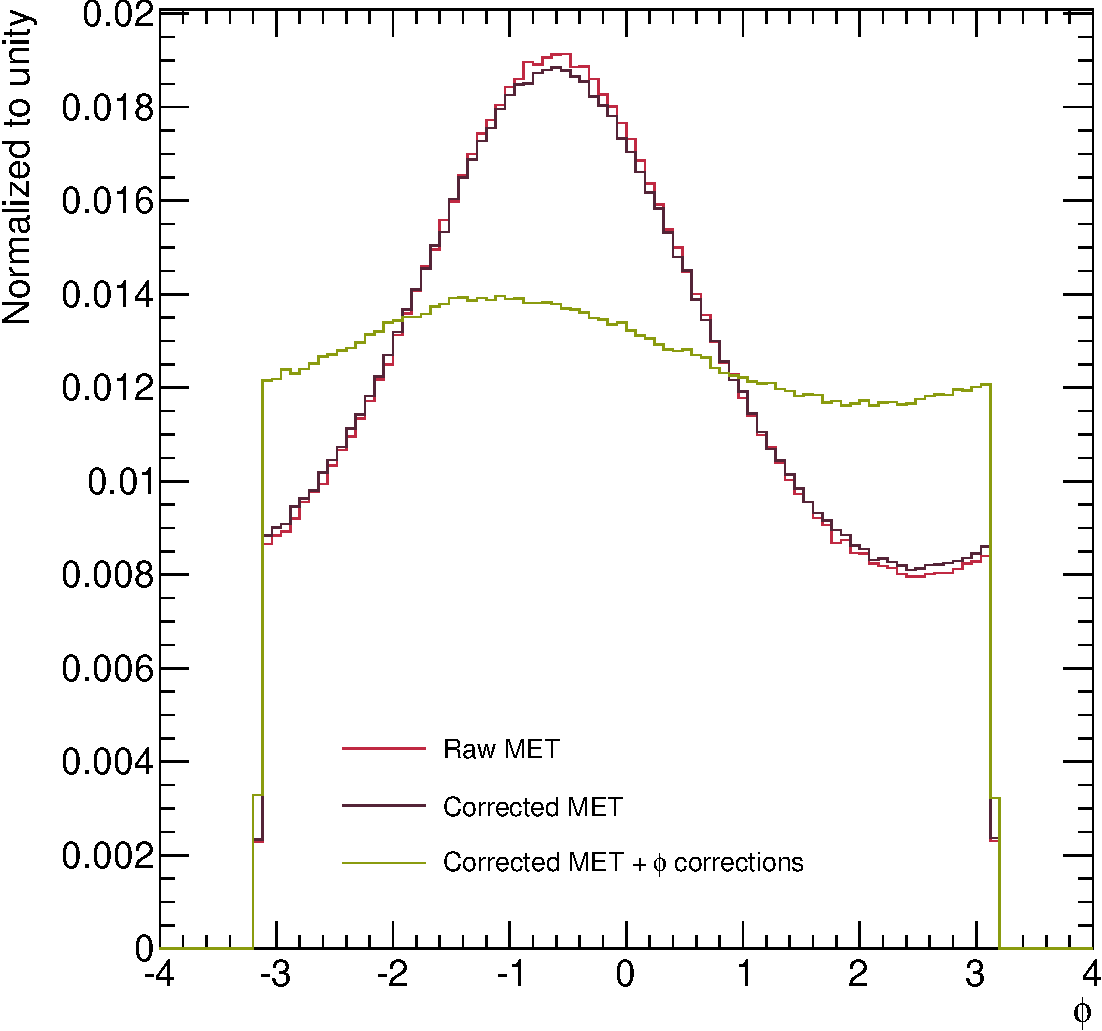
\includegraphics[width=0.48\textwidth]{chapitre7/figs/met_phi_corrections.pdf}}
    \subcaptionbox{\label{fig:met_cleaning}}[0.48\textwidth]{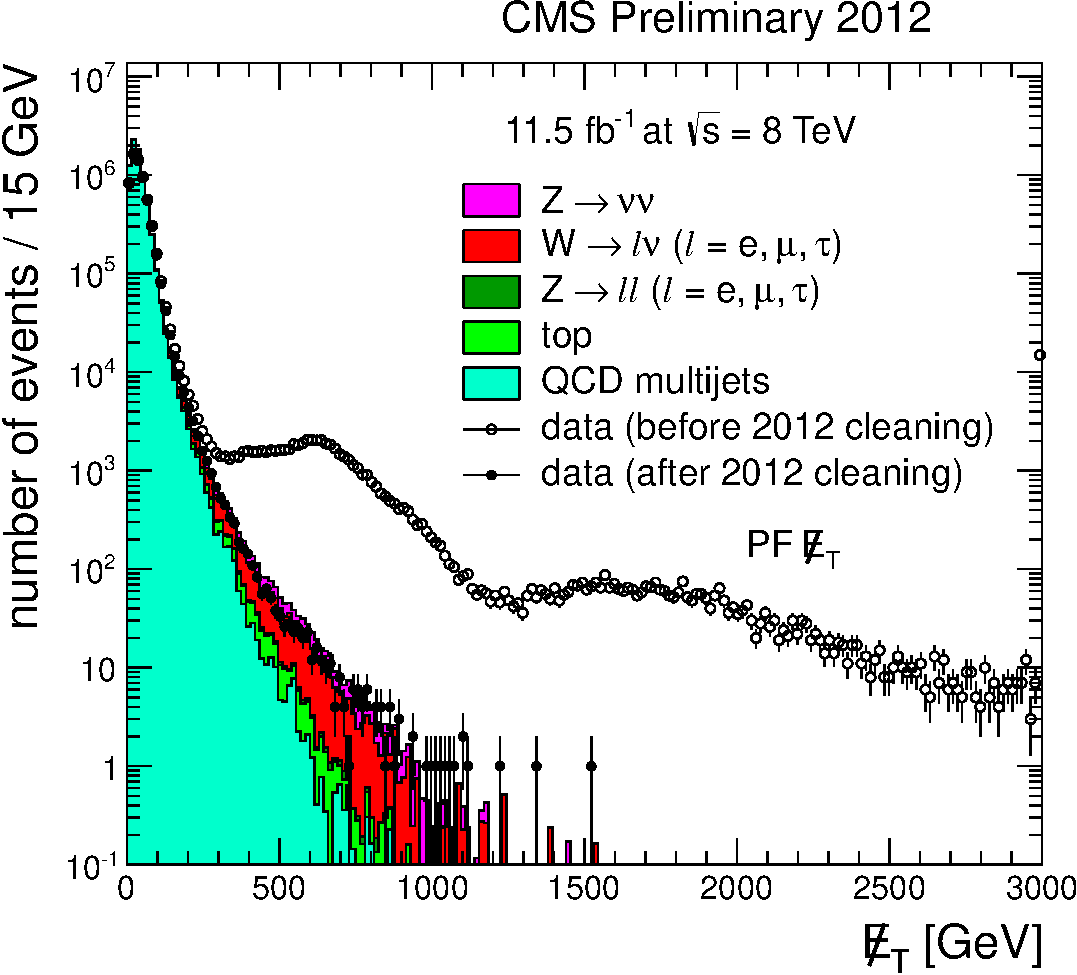
\includegraphics[width=0.48\textwidth]{chapitre7/figs/met_cleaning.pdf}}
    \caption{(\subref{fig:met_phi}) Oscillation en $\phi$ de l'énergie transverse manquante, sans aucune correction (\rouge), après propagation de la correction en énergie des jets (\violet), et après corrections dédiées à l'oscillation en $\phi$ (\vertc). (\subref{fig:met_cleaning}) Effet du nettoyage des données 2012 sur l'énergie transverse manquante.}
\end{figure}

Lors de l'analyse des données 2011, certains événements contenaient une quantité anormalement grande d'énergie transverse manquante. Cette fausse énergie manquante a plusieurs origines :
\begin{itemize}
  \item Des collisions peuvent se produire entre les protons des faisceaux et le gaz résiduel dans les tubes transportant les protons. Dans de rare cas, ces particules peuvent traverser le détecteur, et ainsi apparaître comme de l'énergie transverse manquante.
  \item Du bruit anormal dans le HCAL, causé des problèmes de lecture des photodiodes, peut provoquer de la fausse énergie manquante jusqu'à l'échelle du \si{\TeV}.
  \item Il arrive que le système de synchronisation temporelle du HCAL, utilisant un faisceau laser, se déclenche en même temps qu'une collision. Ce phénomène est extrêmement rare (en 2011, 216 événements ont été identifiés), mais peut causer de grandes valeurs d'énergie transverse manquante.
  \item Certains cristaux du ECAL sont connus pour être très bruyant. Ils sont donc ignorés lors de la reconstruction. Beaucoup d'énergie peut ainsi être manqué lorsqu'une particule interagie avec ces cristaux, provoquant une source anormale d'énergie transverse manquante.
\end{itemize}

Des filtres ont ainsi été développés afin de supprimer les événements contenant de la fausse énergie transverse manquante. On peut voir sur la \cref{fig:met_cleaning} l'effet d'un tel nettoyage : avec l'utilisation des filtres, la queue de la distribution, causée par de la fausse \met, disparaît.

\subsection{Sélection des événements}

Les données collectées par CMS sont classées dans plusieurs ensembles selon les chemins de déclenchements activés. Pour cette analyse, la totalité des données collectées en 2012 est utilisée, correspond à une luminosité intégrée totale de \SI{19.6}{\invfb}. Deux ensembles de données particulier sont utilisés :
\begin{itemize}
  \item L'ensemble \emph{SingleMu}, pour le canal semi-muonique.
  \item L'ensemble \emph{SingleElectron}, pour le canal semi-électronique.
\end{itemize}

On souhaite sélectionner des événements ayant un lepton isolé ainsi qu'au moins 4 jets. Afin de baisser au maximum les seuils en impulsion transverse sur les chemins de déclenchements, on demande aux données d'avoir activé les chemins de déclenchements demandant un lepton isolé et au moins 3 jets centraux ($\aeta < \num{2.5}$). On arrive ainsi à obtenir des chemins de déclenchements demandant un muon isolé d'au moins \SI{17}{\GeV} ou un électron isolé d'au moins \SI{25}{\GeV}, accompagnés d'au moins trois jets d'au moins \SI{30}{\GeV}. Les conditions de prises de données ayant changées pendant l'année 2012, les seuils sur les jets des chemins de déclenchements ont dû être ajustés. Ainsi, on demande au final 4 chemins différents pour le canal semi-muonique et 4 pour le canal semi-électronique. Dans les figures qui suivent, ces chemins ont pour alias respectivement \texttt{HLT\_MuX} (\texttt{HLT\_EleX}), X = A, B, C et D.

\bigskip

La sélection appliquée pour chaque canal est identique, excepté la saveur du lepton demandé. Pour être sélectionné, une événement doit contenir :

\begin{itemize}
  \item Exactement un muon (électron) de qualité, suivant les critères définis \cref{sec:sel_muon} (\cref{sec:sel_electron}). L'événement est rejeté s'il contient en plus un ou plusieurs leptons vérifiant les conditions \textbf{lâches}.
  \item Au moins 4 jets avec $\aeta < \num{2.4}$ et $\pt > 70\,/\,50\,/\,30\,/\,\SI{30}{\GeV}$. Cette coupure étagée permet d'optimiser le rapport signal sur bruit.
  \item Au moins 1 jet étiqueté \Pbottom.
  \item $\met > \SI{20}{\GeV}$. Cette coupure permet d'éliminer une majorité du fond multi-jets.
\end{itemize}

Les événements passant la sélection sont ensuite classés en 4 catégories, selon la saveur du lepton et le nombre de jets étiquetés \Pbottom :
\begin{center}
  \begin{tabular}{@{}c@{}} \toprule
    muon \\
    électron \\ \bottomrule
  \end{tabular} \qquad \times \qquad
  \begin{tabular}{@{}c@{}} \toprule
    1 jet étiqueté \Pbottom \\
    Au moins 2 jets étiquetés \Pbottom \\ \bottomrule
  \end{tabular}
\end{center}

\section{Performances de la sélection}

\subsection{Efficacité des chemins de déclenchements}

Les chemins de déclenchements ne sont pas correctement simulé. En effet, les conditions de prises de données, et donc les différents seuils de chaque chemin, les facteurs de préscale, etc. ne sont pas connues au moment de la génération de la simulation.

Afin d'estimer au mieux l'efficacité des chemins de déclenchements utilisés par l'analyse, chaque chemin a été re-simulé individuellement pour chaque point de signal considéré. Il est ainsi possible d'évaluer l'efficacité de chaque chemin.

Un facteur de correction additionnel est appliqué à chaque efficacité pour tenir compte des différences de performances entre la simulation des chemins et les données. Ces facteurs sont calculés centralement par la collaboration avec une sélection identique pour les leptons, mais légèrement différente (plus lâche) pour les jets. La \cref{fig:trig_eff} présente un exemple de courbes d'efficacités pour les chemins de déclenchement utilisés dans l'analyse. On peut constater que les coupures appliquées sur les jets permettent d'être sur le plateau d'efficacité des chemins. On peut ainsi utiliser une efficacité non dépendante de l'impulsion transverse des objets. Les \cref{tab:HLT_mu_eff_2btag,tab:HLT_mu_eff_1btag,tab:HLT_el_eff_2btag,tab:HLT_el_eff_1btag} résument les efficacités obtenus pour chaque chemin de déclenchement, et pour chacune des catégories de l'analyse. Pour la canal semi-muonique, l'efficacité moyenne est d'environ \SI{90}{\%}, et environ \SI{95}{\%} pour le canal semi-électronique.

\begin{figure}[tbp] \centering
    \subcaptionbox{Canal semi-muonique}[0.48\textwidth]{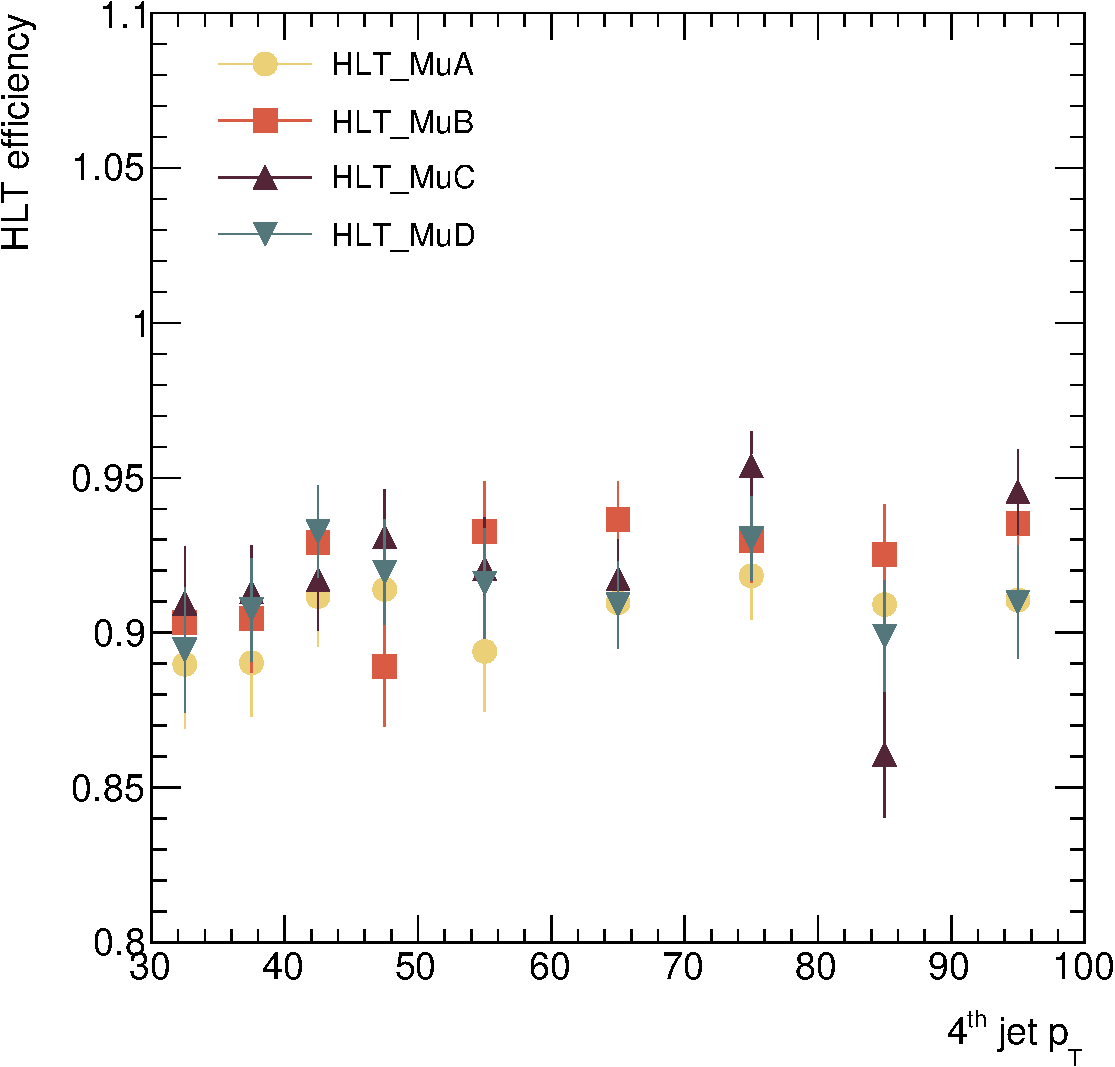
\includegraphics[width=0.48\textwidth]{chapitre7/figs/HLT/HLTturnon_mu_fourthJet_zoom.pdf}}
    \subcaptionbox{Canal semi-électronique}[0.48\textwidth]{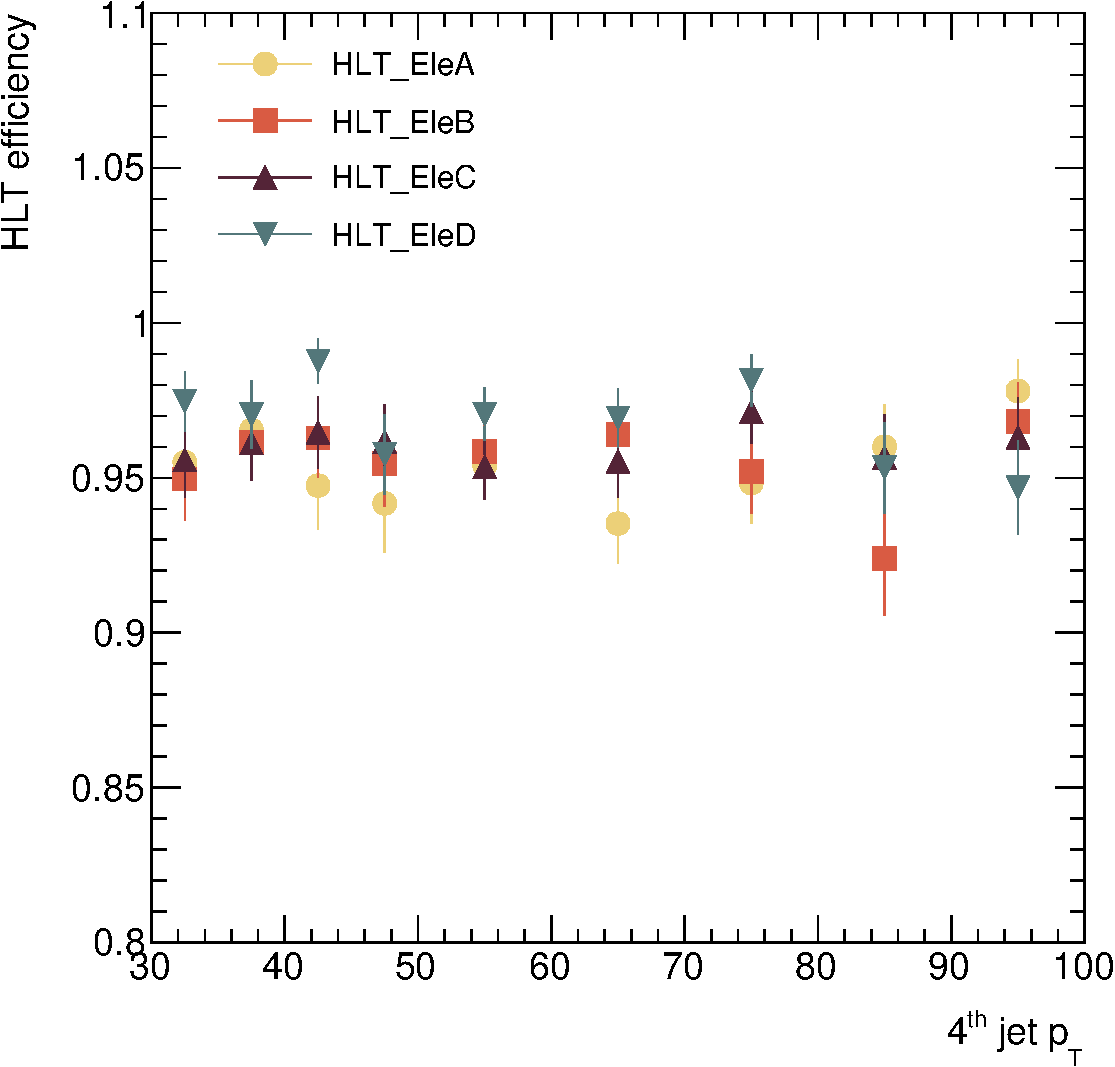
\includegraphics[width=0.48\textwidth]{chapitre7/figs/HLT/HLTturnon_el_fourthJet_zoom.pdf}}
    \caption{Efficacité des chemins de déclenchements en fonction de l'impulsion transverse du quatrième jet.}
    \label{fig:trig_eff}
\end{figure}

% \begin{figure}[tbp] \centering
%     \subcaptionbox{Canal semi-muonique}[0.48\textwidth]{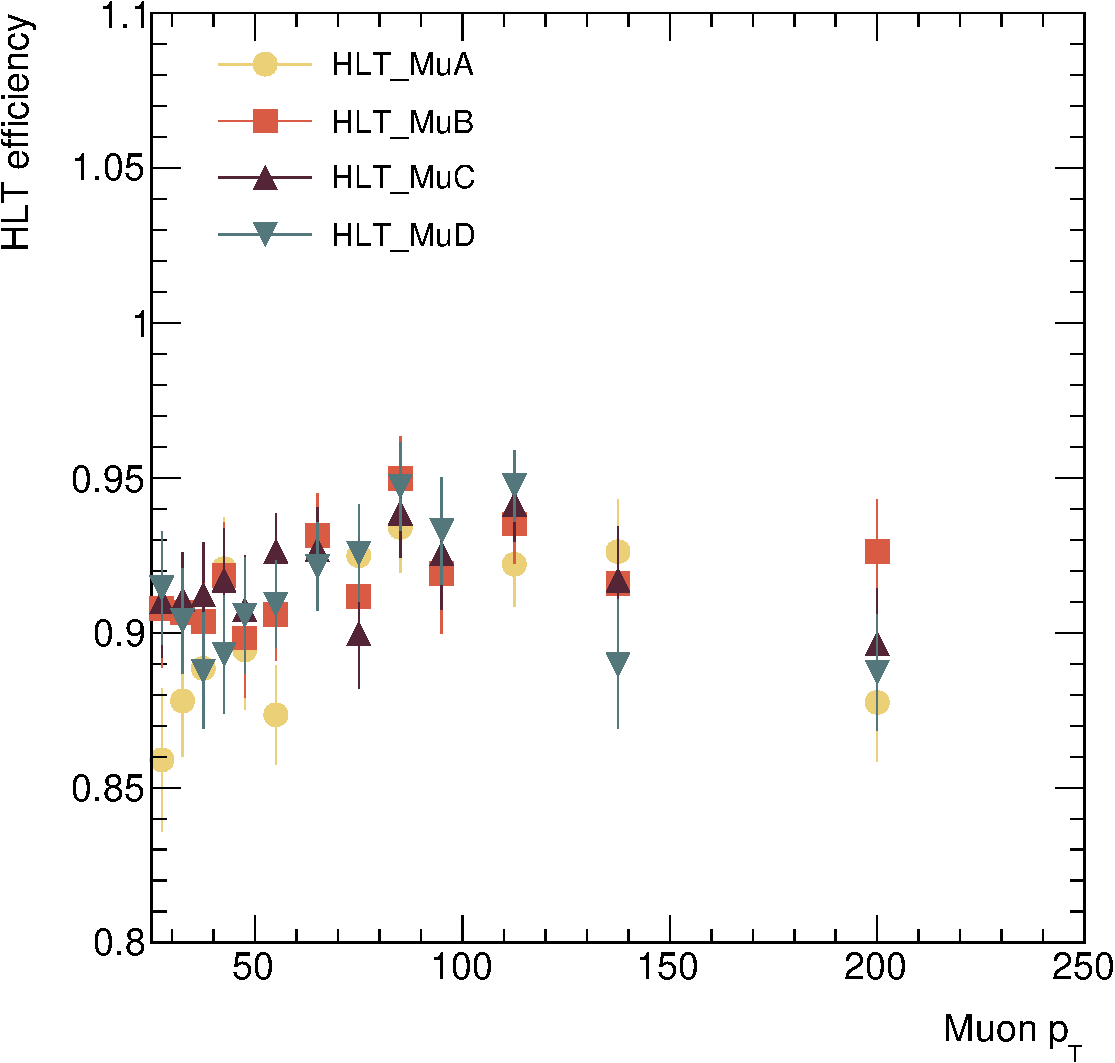
\includegraphics[width=0.48\textwidth]{chapitre7/figs/HLT/HLTturnon_mu_lepton_zoom.pdf}}
%     \subcaptionbox{Canal semi-électronique}[0.48\textwidth]{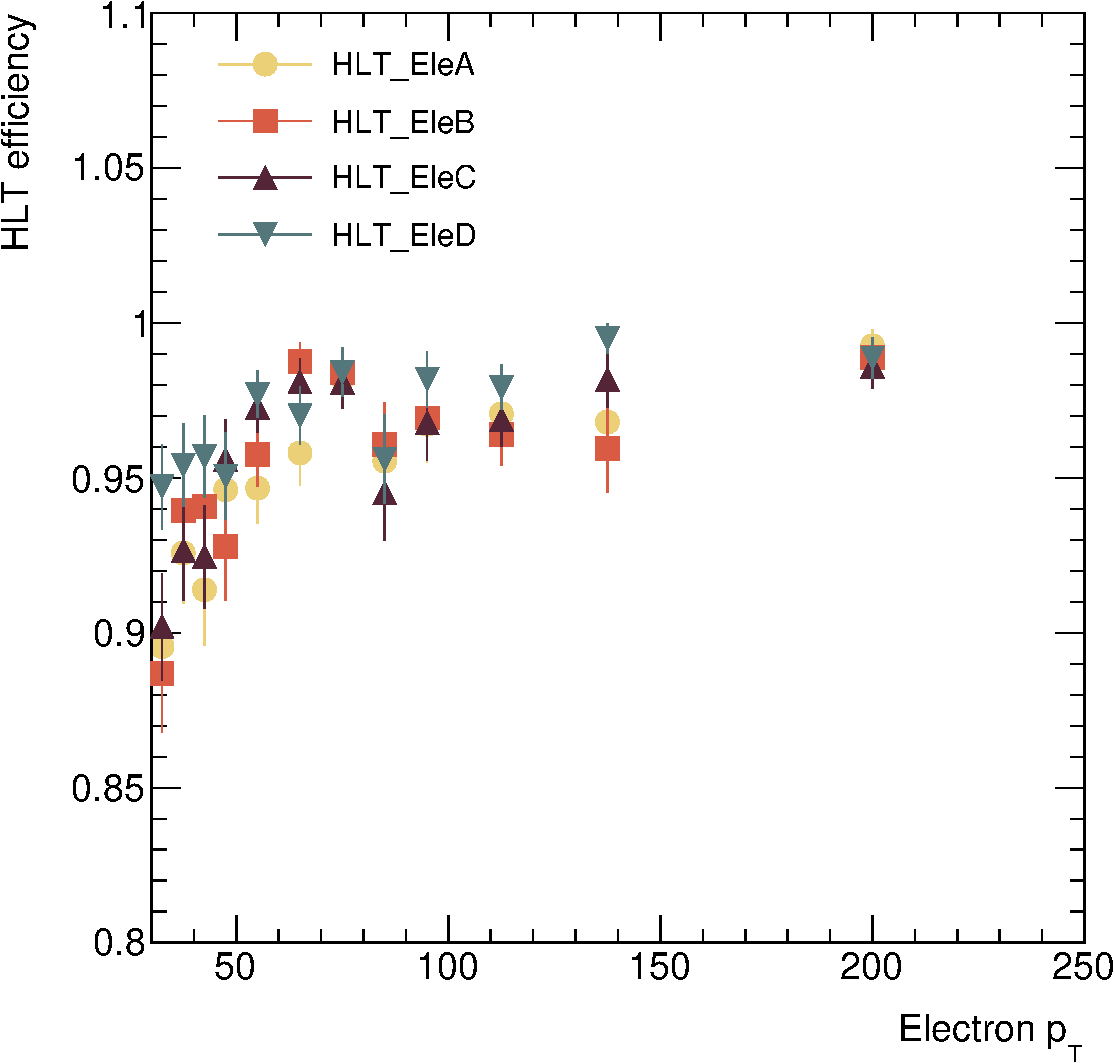
\includegraphics[width=0.48\textwidth]{chapitre7/figs/HLT/HLTturnon_el_lepton_zoom.pdf}}
%     \caption{Efficacité des chemins de déclenchements en fonction de l'impulsion transverse du lepton.}
%     \label{fig:trig_eff_leptons}
% \end{figure}

% \begin{figure}[tbp] \centering
%     \subcaptionbox{\ordinalnum{1} jet}[0.48\textwidth]{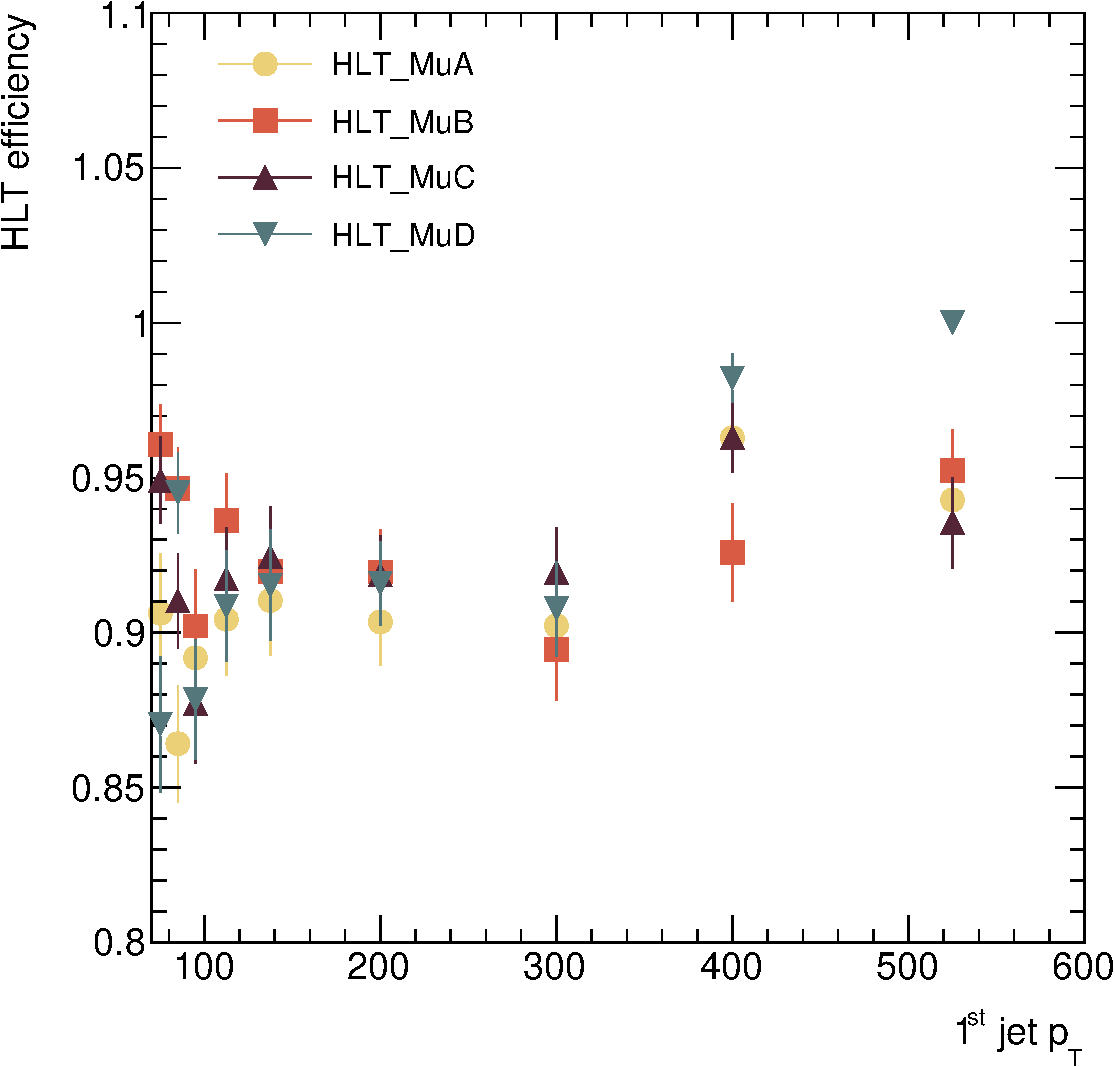
\includegraphics[width=0.48\textwidth]{chapitre7/figs/HLT/HLTturnon_mu_firstJet_zoom.pdf}} \hfill
%     \subcaptionbox{\ordinalnum{2} jet}[0.48\textwidth]{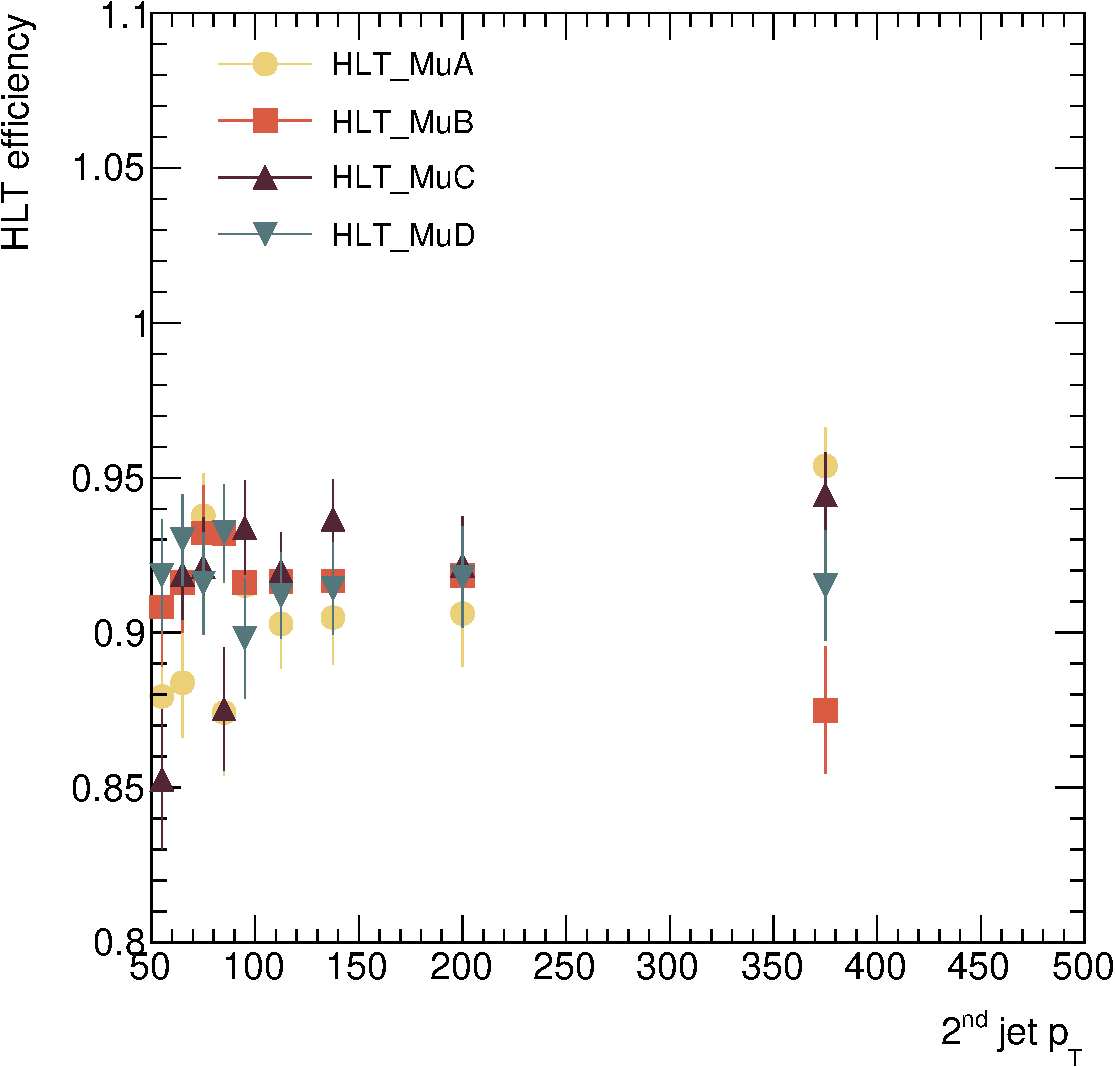
\includegraphics[width=0.48\textwidth]{chapitre7/figs/HLT/HLTturnon_mu_secondJet_zoom.pdf}} \\
%     \subcaptionbox{\ordinalnum{3} jet}[0.48\textwidth]{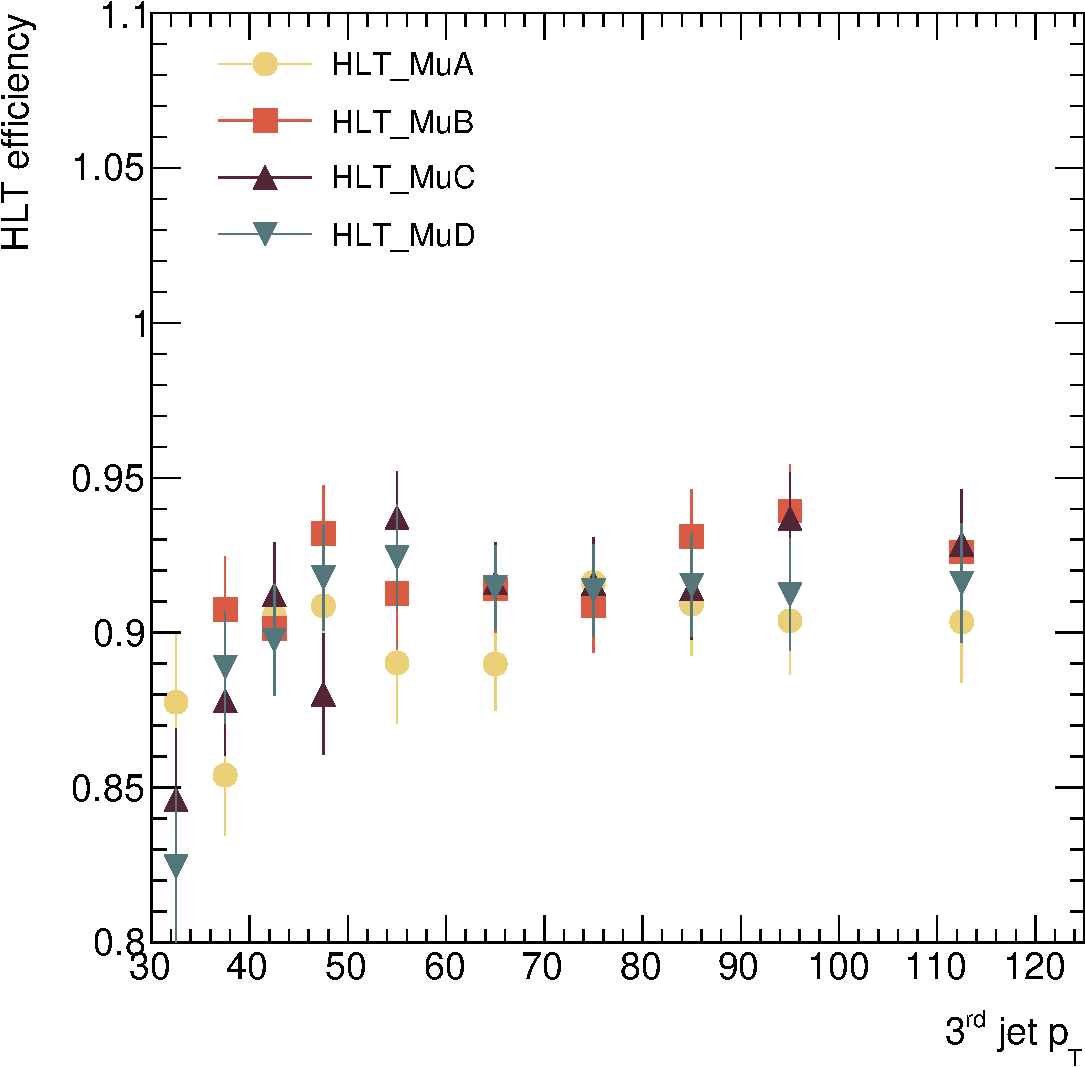
\includegraphics[width=0.48\textwidth]{chapitre7/figs/HLT/HLTturnon_mu_thirdJet_zoom.pdf}} \hfill
%     \subcaptionbox{\ordinalnum{4} jet}[0.48\textwidth]{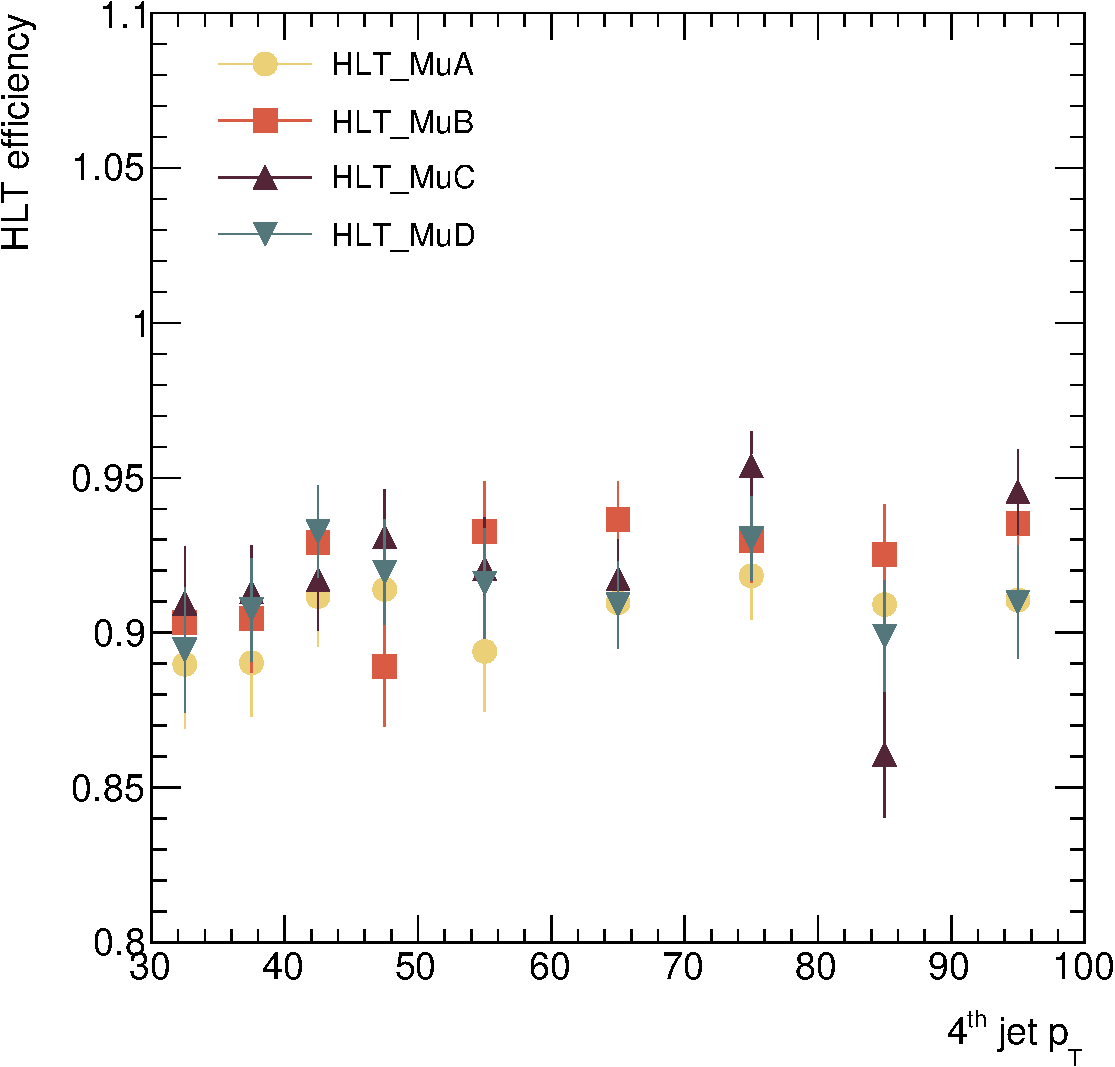
\includegraphics[width=0.48\textwidth]{chapitre7/figs/HLT/HLTturnon_mu_fourthJet_zoom.pdf}}
%     \caption{Efficacité des chemins de déclenchements en fonction de l'impulsion des quatre premiers jets de l'événement pour le canal semi-muonique.}
%     \label{fig:trig_eff_mu_jets}
% \end{figure}

% \begin{figure}[tbp] \centering
%     \subcaptionbox{\ordinalnum{1} jet}[0.48\textwidth]{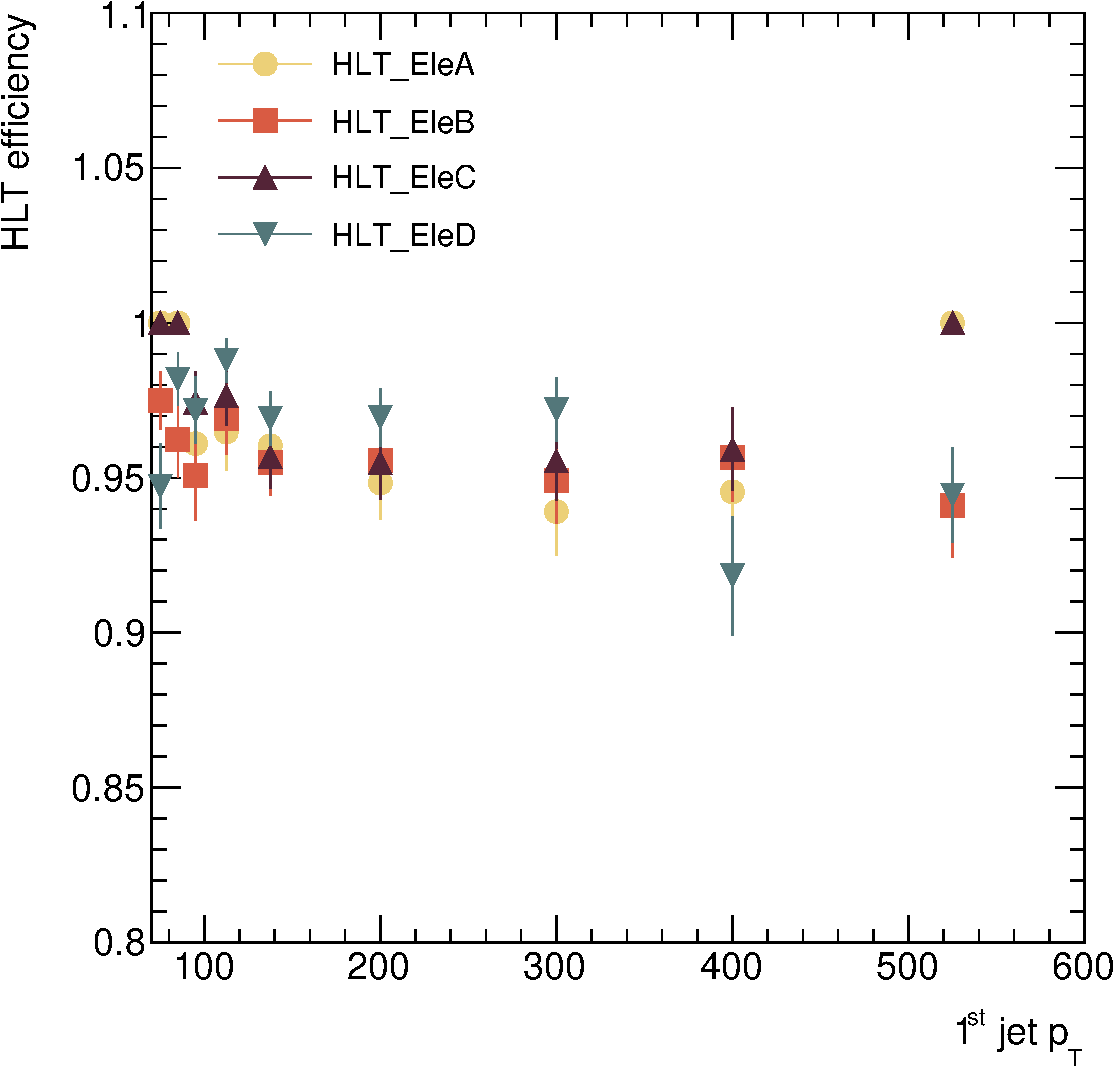
\includegraphics[width=0.48\textwidth]{chapitre7/figs/HLT/HLTturnon_el_firstJet_zoom.pdf}} \hfill
%     \subcaptionbox{\ordinalnum{2} jet}[0.48\textwidth]{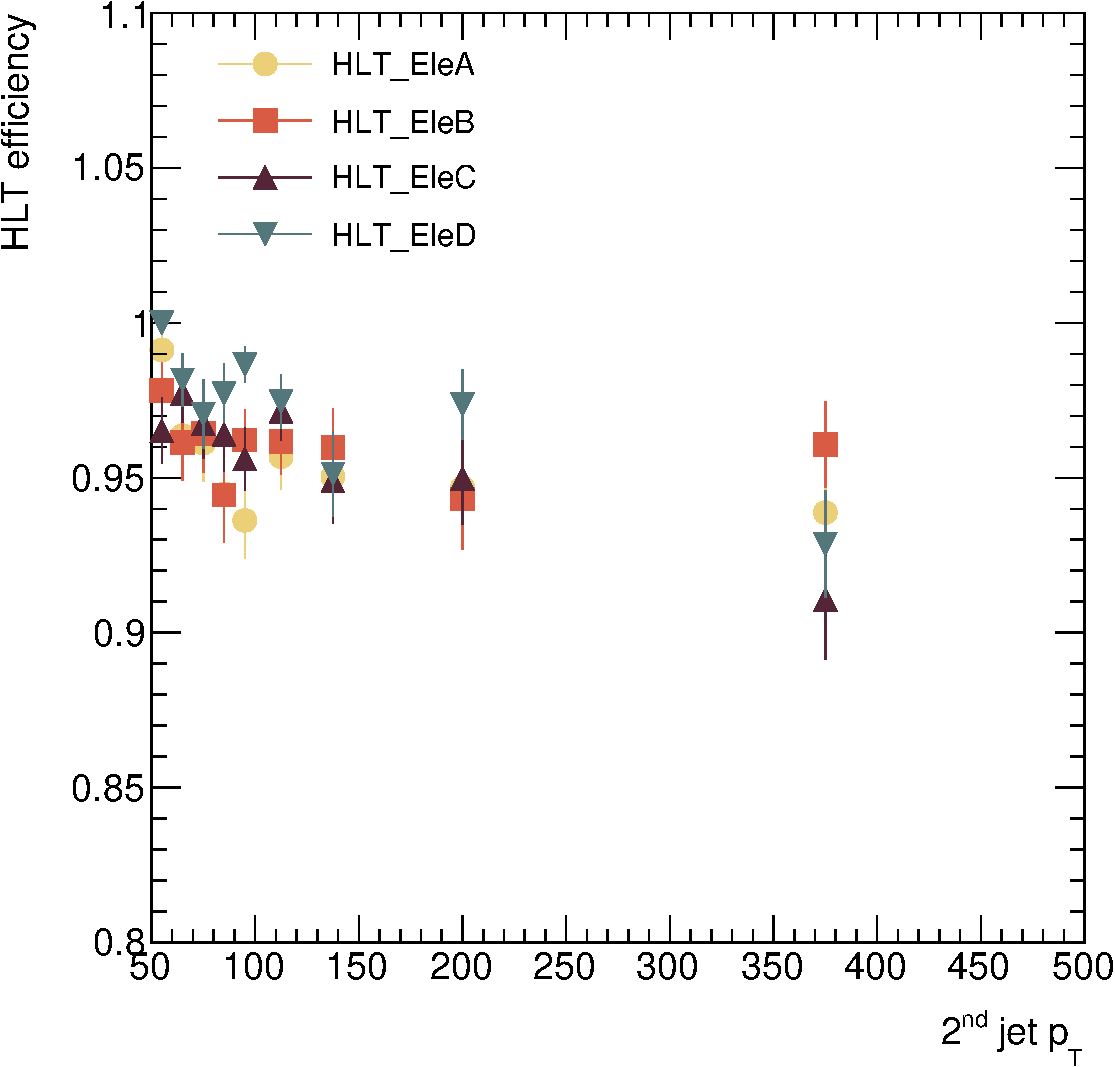
\includegraphics[width=0.48\textwidth]{chapitre7/figs/HLT/HLTturnon_el_secondJet_zoom.pdf}} \\
%     \subcaptionbox{\ordinalnum{3} jet}[0.48\textwidth]{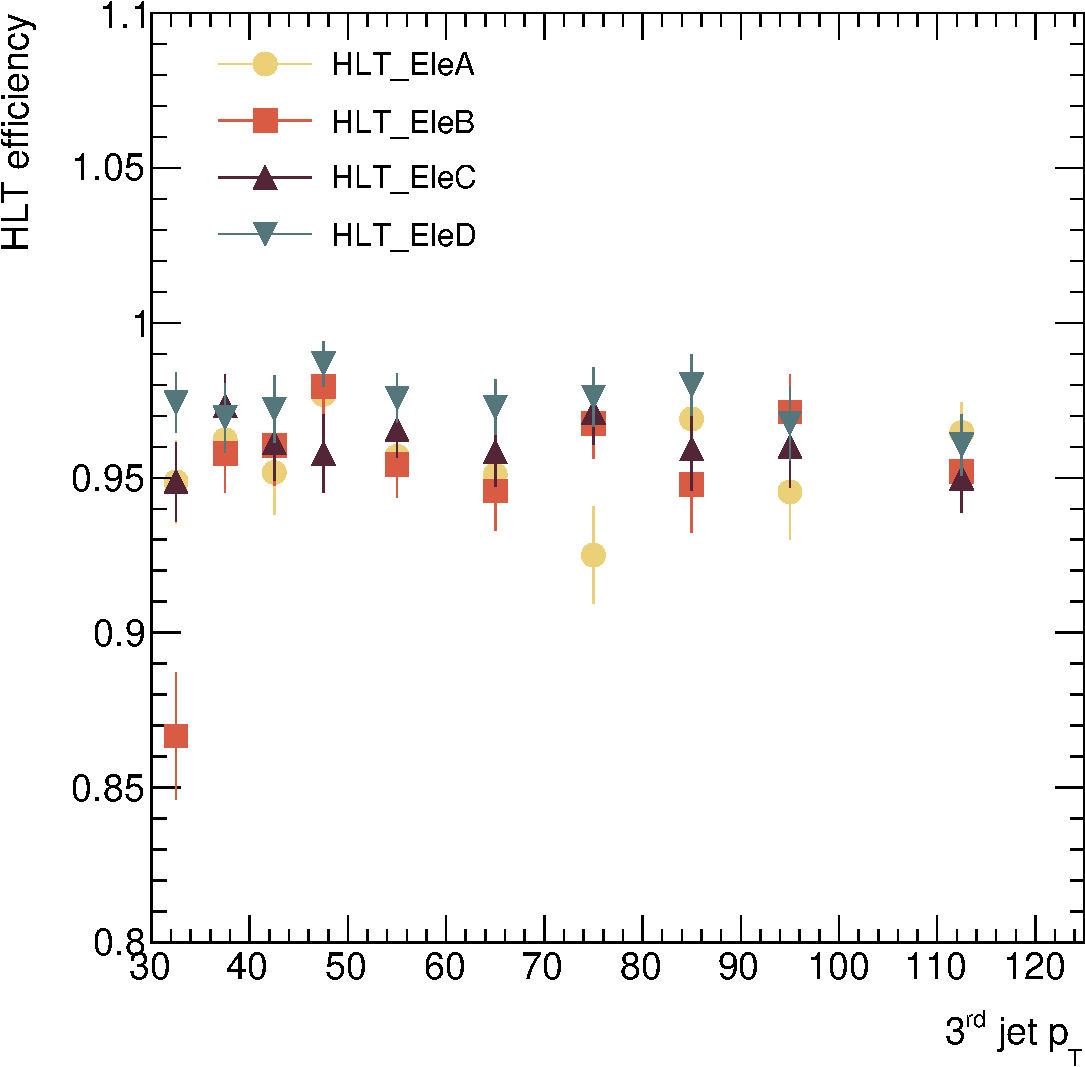
\includegraphics[width=0.48\textwidth]{chapitre7/figs/HLT/HLTturnon_el_thirdJet_zoom.pdf}} \hfill
%     \subcaptionbox{\ordinalnum{4} jet}[0.48\textwidth]{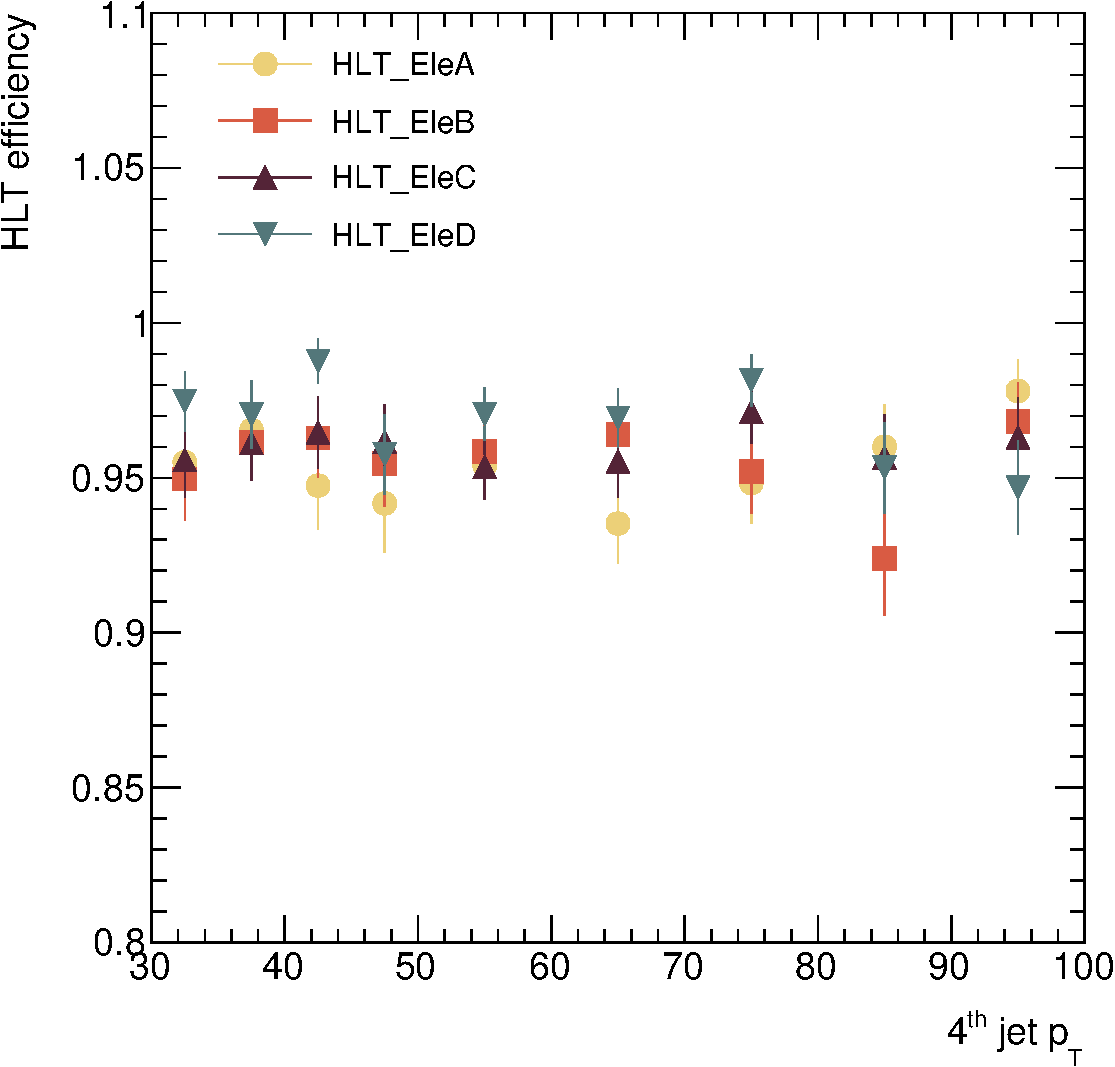
\includegraphics[width=0.48\textwidth]{chapitre7/figs/HLT/HLTturnon_el_fourthJet_zoom.pdf}}
%     \caption{Efficacité des chemins de déclenchements en fonction de l'impulsion des quatre premiers jets de l'événement pour le canal semi-électronique.}
%     \label{fig:trig_eff_e_jets}
% \end{figure}

\begin{table}[p] \centering \footnotesize
\begin{tabular}{@{}ccccc@{}} \toprule
 & \texttt{HLT\_MuA} & \texttt{HLT\_MuB} & \texttt{HLT\_MuC} & \texttt{HLT\_MuD} \\ \midrule
$\epsilon$ ($\mzp = \SI{750}{\GeV}$)& \num{0.909\pm 0.006} & \num{0.909\pm 0.006}& \num{0.917\pm 0.006} & \num{0.909\pm 0.006} \\
$\epsilon$ ($\mzp = \SI{1000}{\GeV}$)& \num{0.899\pm 0.007} & \num{0.916\pm 0.006} & \num{0.928\pm 0.006} & \num{0.918\pm 0.006} \\
$\epsilon$ ($\mzp = \SI{1250}{\GeV}$)& \num{0.889\pm 0.008} & \num{0.908\pm 0.007} & \num{0.904\pm 0.007} & \num{0.908\pm 0.007} \\
$\epsilon$ ($\mzp = \SI{1500}{\GeV}$)& \num{0.900\pm 0.008} & \num{0.908\pm 0.008} & \num{0.904\pm 0.008} & \num{0.930\pm 0.007} \\
$\epsilon$ (\ttbar)& \num{0.891\pm 0.006} & \num{0.912\pm 0.006} & \num{0.915\pm 0.006} & \num{0.929\pm 0.006} \\ \hline
\end{tabular}
\caption{Efficacités des chemins de déclenchements pour le canal semi-muonique, et au moins 2 jets étiquetés \Pbottom.}
\label{tab:HLT_mu_eff_2btag}
\end{table}

\begin{table}[p] \centering \footnotesize
\begin{tabular}{@{}ccccc@{}} \toprule
 & \texttt{HLT\_MuA} & \texttt{HLT\_MuB} & \texttt{HLT\_MuC} & \texttt{HLT\_MuD} \\ \midrule
$\epsilon$ ($\mzp = \SI{750}{\GeV}$)& \num{0.902\pm 0.007} & \num{0.920\pm 0.006} & \num{0.921\pm 0.006} & \num{0.913\pm0.007} \\
$\epsilon$ ($\mzp = \SI{1000}{\GeV}$)& \num{0.897\pm 0.007} & \num{0.918\pm 0.006} & \num{0.917\pm 0.006} & \num{0.922\pm 0.006} \\
$\epsilon$ ($\mzp = \SI{1250}{\GeV}$)& \num{0.899\pm 0.008} & \num{0.904\pm 0.007} & \num{0.902\pm 0.007} & \num{0.919\pm 0.006} \\
$\epsilon$ ($\mzp = \SI{1500}{\GeV}$)& \num{0.902\pm 0.007} & \num{0.910\pm 0.008} & \num{0.919\pm 0.007} & \num{0.925\pm 0.007} \\
$\epsilon$ (\ttbar)& \num{0.883\pm 0.006} & \num{0.915\pm 0.006} & \num{0.913\pm 0.006} & \num{0.919\pm 0.006} \\ \hline
\end{tabular}
\caption{Efficacités des chemins de déclenchements pour le canal semi-muonique, et exactement 1 jet étiqueté \Pbottom.}
\label{tab:HLT_mu_eff_1btag}
\end{table}

\begin{table}[p] \centering \footnotesize
\begin{tabular}{@{}ccccc@{}} \toprule
 & \texttt{HLT\_EleA} & \texttt{HLT\_EleB} & \texttt{HLT\_EleC} & \texttt{HLT\_EleD} \\ \midrule
$\epsilon$ ($\mzp = \SI{750}{\GeV}$)& \num{0.955\pm 0.005} & \num{0.956\pm 0.005} & \num{0.958\pm 0.005} & \num{0.966\pm0.005} \\
$\epsilon$ ($\mzp = \SI{1000}{\GeV}$)& \num{0.968\pm 0.004} & \num{0.962\pm 0.005} & \num{0.966\pm 0.004} & \num{0.975\pm 0.004} \\
$\epsilon$ ($\mzp = \SI{1250}{\GeV}$)& \num{0.958\pm 0.005} & \num{0.957\pm 0.005} & \num{0.958\pm 0.005} & \num{0.964\pm 0.005} \\
$\epsilon$ ($\mzp = \SI{1500}{\GeV}$)& \num{0.955\pm 0.006} & \num{0.954\pm 0.006} & \num{0.950\pm 0.006} & \num{0.963\pm 0.005} \\
$\epsilon$ (\ttbar)& \num{0.956\pm 0.005} & \num{0.960\pm 0.004} & \num{0.958\pm 0.004} & \num{0.973\pm 0.004}  \\ \hline
\end{tabular}
\caption{Efficacités des chemins de déclenchements pour le canal semi-électronique, et au moins 2 jets étiquetés \Pbottom.}
\label{tab:HLT_el_eff_2btag}
\end{table}

\begin{table}[p] \centering \footnotesize
\begin{tabular}{@{}ccccc@{}} \toprule
 & \texttt{HLT\_EleA} & \texttt{HLT\_EleB} & \texttt{HLT\_EleC} & \texttt{HLT\_EleD} \\ \midrule
$\epsilon$ ($\mzp = \SI{750}{\GeV}$)& \num{0.949\pm 0.005} & \num{0.954\pm 0.005} & \num{0.960\pm 0.005} & \num{0.976\pm0.004} \\
$\epsilon$ ($\mzp = \SI{1000}{\GeV}$)& \num{0.950\pm 0.005} & \num{0.962\pm 0.005} & \num{0.957\pm 0.005} & \num{0.960\pm 0.005} \\
$\epsilon$ ($\mzp = \SI{1250}{\GeV}$)& \num{0.958\pm 0.005} & \num{0.947\pm 0.005} & \num{0.962\pm 0.005} & \num{0.963\pm 0.004} \\
$\epsilon$ ($\mzp = \SI{1500}{\GeV}$)& \num{0.945\pm 0.005} & \num{0.932\pm 0.006} & \num{0.946\pm 0.006} & \num{0.960\pm 0.005} \\
$\epsilon$ (\ttbar)& \num{0.956\pm 0.005} & \num{0.954\pm 0.004} & \num{0.957\pm 0.004} & \num{0.968\pm 0.004} \\ \hline
\end{tabular}
\caption{Efficacités des chemins de déclenchements pour le canal semi-électronique, et exactement 1 jet étiqueté \Pbottom.}
\label{tab:HLT_el_eff_1btag}
\end{table}

\subsection{Efficacité de sélection}

Les \cref{tab:eff_narrow_1b,tab:eff_narrow_2b} présentent les efficacités de sélection pour différentes masses de \zprime dans l'hypothèse de résonances étroites et pour les 4 catégories de l'analyse. Ces efficacités sont inclusives, c'est-à-dire calculées en considérant tous les canaux de désintégrations des paires \ttbar, et pas seulement le canal semi-leptonique. De façon équivalente, les efficacités obtenues dans le cas de \zprime larges sont résumées dans les \cref{tab:eff_large_1b,tab:eff_large_2b}. Toutes ces efficacités sont calculées après avoir appliqué une coupure supplémentaire $\mtt > \SI{550}{\GeV}$ (les raisons d'un tel choix sont décrites plus loin dans ce chapitre). Cette coupure explique pourquoi l'efficacité de sélection pour la résonance à \SI{500}{\GeV} est si faible comparé aux autres masses.

\bigskip

Afin d'obtenir l'efficacité d'un éventuel signal sur les données, des facteurs de corrections sont appliqués pour tenir compte des différences de performances de l'algorithme d'étiquetage des \Pbottom ainsi que l'efficacité d'identification et d'isolation des leptons entre la simulation et les données. Ces facteurs de corrections sont calculés centralement par la collaboration, et dépendent de l'impulsion transverse et de la pseudo-rapidité des objets physiques concernés. Pour obtenir un facteur de correction global à appliquer aux efficacités de sélection, les valeurs centrales sont combinées en tenant compte des spectres en \pt et \aeta des objets physique du signal. On obtient au final les facteurs de corrections suivants :
\begin{itemize}
  \item Identification et isolation des muons : \num{0.992 \pm 0.005}.
  \item Identification et isolation des électrons : \num{0.982 \pm 0.003}.
  \item Étiquetage des jets de \Pbottom : \num{1.043 \pm 0.022} pour exactement 1 jet étiqueté \Pbottom, et \num{0.927 \pm 0.038} pour au moins deux jets étiquetés \Pbottom.
\end{itemize}

\begin{table}[p] \centering
  \begin{tabular}{ccccccc} \toprule
    & \SI{500}{\GeV} & \SI{750}{\GeV} & \SI{1000}{\GeV} & \SI{1250}{\GeV} & \SI{1500}{\GeV} & \SI{2000}{\GeV} \\ \midrule
    $\epsilon$, semi-$\mu$ & \num{0.55 \pm 0.02} & \num{1.60 \pm 0.03} & \num{1.87 \pm 0.03} & \num{1.86 \pm 0.03} & \num{1.63 \pm 0.03} & \num{1.13 \pm 0.02} \\
    $\epsilon$, semi-e & \num{0.47 \pm 0.01} & \num{1.43 \pm 0.03} & \num{1.74 \pm 0.03} & \num{1.80 \pm 0.03} & \num{1.61 \pm 0.03} & \num{1.22 \pm 0.03} \\ \bottomrule
  \end{tabular}
  \caption{Efficacités de sélection du signal pour différentes masses de \zprime dans l'hypothèse de résonances étroites, en demandant exactement 1 jet étiqueté \Pbottom. Ces efficacités sont calculés par rapport à la désintégration $\zprime \rightarrow \ttbar$ inclusive.}
  \label{tab:eff_narrow_1b}
\end{table}

\begin{table}[p] \centering
  \begin{tabular}{ccccccc} \toprule
    & \SI{500}{\GeV} & \SI{750}{\GeV} & \SI{1000}{\GeV} & \SI{1250}{\GeV} & \SI{1500}{\GeV} & \SI{2000}{\GeV} \\ \midrule
    $\epsilon$, semi-$\mu$ & \num{0.51 \pm 0.01} & \num{1.62 \pm 0.03} & \num{1.90 \pm 0.03} & \num{1.67 \pm 0.03} & \num{1.38 \pm 0.03} & \num{0.81 \pm 0.02} \\
    $\epsilon$, semi-e & \num{0.43 \pm 0.01} & \num{1.46 \pm 0.03} & \num{1.68 \pm 0.03} & \num{1.57 \pm 0.03} & \num{1.32 \pm 0.03} & \num{0.81 \pm 0.02} \\ \bottomrule
  \end{tabular}
  \caption{Efficacités de sélection du signal pour différentes masses de \zprime dans l'hypothèse de résonances étroites, en demandant au moins 2 jets étiquetés \Pbottom. Ces efficacités sont calculés par rapport à la désintégration $\zprime \rightarrow \ttbar$ inclusive.}
  \label{tab:eff_narrow_2b}
\end{table}

\begin{table}[p] \centering
  \begin{tabular}{ccccccc} \toprule
    & \SI{500}{\GeV} & \SI{750}{\GeV} & \SI{1000}{\GeV} & \SI{1250}{\GeV} & \SI{1500}{\GeV} & \SI{2000}{\GeV} \\ \midrule
    $\epsilon$, semi-$\mu$ & \num{0.66 \pm 0.02} & \num{1.57 \pm 0.03} & \num{1.89 \pm 0.03} & \num{1.81 \pm 0.03} & \num{1.65 \pm 0.03} & \num{1.31 \pm 0.03} \\
    $\epsilon$, semi-e & \num{0.48 \pm 0.02} & \num{1.25 \pm 0.02} & \num{1.63 \pm 0.03} & \num{1.60 \pm 0.03} & \num{1.66 \pm 0.03} & \num{1.28 \pm 0.03} \\ \bottomrule
  \end{tabular}
  \caption{Efficacités de sélection du signal pour différentes masses de \zprime dans l'hypothèse de résonances larges, en demandant exactement 1 jet étiqueté \Pbottom. Ces efficacités sont calculés par rapport à la désintégration $\zprime \rightarrow \ttbar$ inclusive.}
  \label{tab:eff_large_1b}
\end{table}

\begin{table}[p] \centering
  \begin{tabular}{ccccccc} \toprule
    & \SI{500}{\GeV} & \SI{750}{\GeV} & \SI{1000}{\GeV} & \SI{1250}{\GeV} & \SI{1500}{\GeV} & \SI{2000}{\GeV} \\ \midrule
    $\epsilon$, semi-$\mu$ & \num{0.62 \pm 0.02} & \num{1.60 \pm 0.03} & \num{1.81 \pm 0.03} & \num{1.64 \pm 0.03} & \num{1.40 \pm 0.03} & \num{1.07 \pm 0.02} \\
    $\epsilon$, semi-e & \num{0.48 \pm 0.02} & \num{1.38 \pm 0.03} & \num{1.55 \pm 0.03} & \num{1.52 \pm 0.04} & \num{1.35 \pm 0.04} & \num{1.02 \pm 0.02} \\ \bottomrule
  \end{tabular}
  \caption{Efficacités de sélection du signal pour différentes masses de \zprime dans l'hypothèse de résonances larges, en demandant au moins 2 jets étiquetés \Pbottom. Ces efficacités sont calculés par rapport à la désintégration $\zprime \rightarrow \ttbar$ inclusive.}
  \label{tab:eff_large_2b}
\end{table}

\section{Reconstruction de la masse invariante}